% interactnlmsample.tex
% v1.05 - August 2017

\documentclass[]{interact}

\newcommand{\red}[1]{{\color{red}#1}}
\usepackage{epstopdf}% To incorporate .eps illustrations using PDFLaTeX, etc.
\usepackage[caption=false]{subfig}% Support for small, `sub' figures and tables
%\usepackage[nolists,tablesfirst]{endfloat}% To `separate' figures and tables from text if required
%\usepackage[doublespacing]{setspace}% To produce a `double spaced' document if required
%\setlength\parindent{24pt}% To increase paragraph indentation when line spacing is doubled
\usepackage{color}
\usepackage{graphicx}
\graphicspath{ {Figures/} }
\usepackage[numbers,sort&compress]{natbib}% Citation support using natbib.sty
\bibpunct[, ]{[}{]}{,}{n}{,}{,}% Citation support using natbib.sty
\renewcommand\bibfont{\fontsize{10}{12}\selectfont}% Bibliography support using natbib.sty
\makeatletter% @ becomes a letter
\def\NAT@def@citea{\def\@citea{\NAT@separator}}% Suppress spaces between citations using natbib.sty
\makeatother% @ becomes a symbol again

\theoremstyle{plain}% Theorem-like structures provided by amsthm.sty
\newtheorem{theorem}{Theorem}[section]
\newtheorem{lemma}[theorem]{Lemma}
\newtheorem{corollary}[theorem]{Corollary}
\newtheorem{proposition}[theorem]{Proposition}

\theoremstyle{definition}
\newtheorem{definition}[theorem]{Definition}
\newtheorem{example}[theorem]{Example}

\theoremstyle{remark}
\newtheorem{remark}{Remark}
\newtheorem{notation}{Notation}


\renewcommand{\arraystretch}{1.2} % please do not remove or change
\newcommand{\cpl}{Chem. Phys. Lett.}
\newcommand{\jpc}{J. Phys. Chem.}
\newcommand{\aap}{Astron. Astrophys.}
\newcommand{\apjl       }{Astrophys. J. Lett.}
\newcommand{\apj       }{Astrophys. J. }
\newcommand{\araa       }{Annu. Rev. Astron. Astrophys.}
\newcommand{\apss       }{?????????????????}                
\newcommand{\jcc        }{J. Comput. Chem.}
\newcommand{\jcompp     }{J. Comput. Phys.}
\newcommand{\apjs       }{Astrophys. J. Suppl.}
\newcommand{\csr        }{Chem. Soc. Rev.}                        
\newcommand{\cpc        }{Comput. Phys. Comm.}                        
\newcommand{\jpcm       }{J. Phys. Condens. Matter}
\newcommand{\ijqm       }{Int. J. Quant. Chem.}
\newcommand{\pccp       }{Phys. Chem. Chem. Phys.}
\newcommand{\molp         }{Mol. Phys.}
\newcommand{\pnas       }{Proc. Natl. Acad. Sci. Unit. States Am.}
\newcommand{\ijms       }{Int. J. Mass Spectrom.} 
\newcommand{\jesrp      }{J. Electron. Spectros. Relat. Phenom.}
\newcommand{\jacs       }{J. Am. Chem. Soc.}              
\newcommand{\baas       }{????????????????????????????}
\newcommand{\mnras      }{           ??????????????????        }
\newcommand{\acp        }{Adv. Chem. Phys.}
\newcommand{\cp         }{Chem. Phys.}
\newcommand{\pr         }{Phys. Rev.}
\newcommand{\epjd       }{Eur. Phys. J. D}
\newcommand{\jpcc       }{J. Phys. Colloid. Chem.}
\newcommand{\hca        }{Helv. Chim. Act.} 
\newcommand{\cms        }{Comput. Mater. Sci.}
\newcommand{\jctc       }{J. Chem. Theor. Comput.}
\newcommand{\eurl       }{Europhys. lett.}       
\newcommand{\ijqc       }{Int. J. Quant. Chem.}     
\newcommand{\dftbpapers}{dftb1,dftb2,scc-dftb,frauenheim00,frauenheim02,augusto09}
\newcommand{\dftcipapers}{Wu05,wu06,const_dft,coupl_dftci,cidft,coupl_dftci,wu09,vanvoorhis10}
\newcommand{\jcp       }{J. Chem. Phys.}       
\newcommand{\prl       }{Phys. Rev. Lett.}    


\begin{document}

\title{Contribution of the Density-Functional based Tight-Binding Scheme to the Description of Water Clusters: Methods, Applications and
Extension to Bulk Systems}

\author{
\name{A. Simon\textsuperscript{a}\thanks{CONTACT A. Simon. Email: aude.simon@irsamc.ups-tlse.fr}, M. Rapacioli\textsuperscript{a}, E. Michoulier\textsuperscript{b}, L. Zheng\textsuperscript{a}, K. Korchagina\textsuperscript{a} and J. Cuny\textsuperscript{a}}
\affil{\textsuperscript{a}Laboratoire de Chimie et Physique Quantiques LCPQ/IRSAMC, Universit\'e de Toulouse and CNRS, UT3-Paul Sabatier,  118 Route de Narbonne, F-31062 Toulouse, France}
\affil{\textsuperscript{b}Laboratoire de Collisions Atomiques et R\'eactivit\'e LCAR/IRSAMC, Universit\'e de Toulouse  and CNRS, UT3-Paul Sabatier, 118 Route de Narbonne, F-31062 Toulouse, France}
}

\maketitle

\begin{abstract}
This review is dedicated to the application of the self-consistent-charge density-functional based tight-binding (SCC-DFTB)
approach to describe the structures, energetics, thermodynamics and spectral properties of water clusters, in the context of both fundamental and applied studies.
We first present modifications implemented in the parametrization of the potential that is
mandatory to describe molecular aggregates. Then a number of applications of atmospherical and astrophysical interest, involving
collaborations between theoreticians and experimentalists, are discussed to exemplify past and present contributions of SCC-DFTB to
those two domains. Most applications presented in this review take advantage of the computational efficiency of SCC-DFTB to
conduct extensive molecular dynamics simulations to obtain spectral and thermodynamical properties of water clusters.  We also show some new results related to ongoing studies on both clusters and liquid water. Some perspectives of our work are also presented, which are in particular heading towards the description of infinite systems such asphaltene molecules and clusters at the solvant-water interface, still in a collaborative context in the framework of petro-chemistry.
\end{abstract}

\begin{keywords}
SCC-DFTB; Water; Cluster; Aggregates; Molecular Dynamics; Proton; PAH
\end{keywords}

\section{Introduction}

The theoretical description of water clusters is an ongoing research topic that has appeared several decades ago
in parallel with the development of experimental set-up designed especially to probe those ubiquitous objects
\cite{Haberland1986,Liu1996a,Paul1997,Paul1999,Buck2000,Keutsch2001,Keutsch2001b}.
The interest for water clusters has then tremendously increased as they can be viewed as models to understand the
behavior of the condensed phases of water \cite{Gregory1997,Keutsch2001a}, ice and liquid, or to rationalize bonding patterns in
hydrogen-bonded species. They are also prototypical systems to study proton transfer processes \cite{Wolke2016}.
These fundamental studies are of paramount importance to understand the key role of water clusters  in atmospheric and interstellar chemistry processes. Indeed, water clusters constitute  an environment  for particle growth in the former case while they may  act as a support to promote  important chemical reactions in the latter case. 

%whether it
%is as support to promote important chemical reactions in the latter case or as medium for particle growth in the
%former one.

Over the years, a proper understanding of the properties of water clusters has required a strong synergy between experimental
and theoretical approaches. Indeed, the structural complexity of the clusters makes it difficult to experimentally rationalize 
their properties without a theoretical support, even at the lowest temperatures. Of course, this especially applies to
medium-size to large species which are characterized by a number of low-energy isomers, see for instance the recent
example of  (H$_{2}$O)$_{11}$ \cite{Temelso2018}. Nevertheless, this is also true for the smallest sizes, as
exemplified by the long standing issue concerning the nature of the lowest-energy isomer of (H$_{2}$O)$_{6}$
\cite{Liu1996,Liu1997,Steinbach2004,Saykally2012,Perez2012}. When temperature increases, the properties of a given aggregate
originate from a variety of isomers, which is very difficult to probe experimentally \cite{Wang2012,Temelso2018} but
can be rationalized using theoretical simulations.

A variety of approaches exist to model bare, protonated, deprotonated or charged water clusters as well as water clusters
interacting with other chemical species such as organic molecules or inorganic ions. This ranges from force fields \cite{Cisneros2016} 
to wavefunction based methods, through semi-empirical models or density functional theory (DFT). Each approach
displays strengths and weaknesses resulting from a different balance between accuracy and computational cost.
Among the whole of available methods, the self-consistent-charge density-functional based tight-binding (SCC-DFTB)
approach presents an interesting compromise between these two criteria. 
Indeed, SCC-DFTB is a quantum chemical method, \textit{i.e.} it provides an explicit description of the electronic structure,
while displaying a rather limited computational cost as compared to wavefunction-based methods or DFT resulting
from several approximations. This allows to combine SCC-DFTB to extensive simulation schemes such as Monte-Carlo (MC)
or molecular dynamics (MD) to explore complex potential energy surfaces (PES) or to derive finite-temperature,
thermodynamic or spectral properties. Over the last ten years, various implementations, corrections and extensions
of SCC-DFTB have been proposed which have been successfully applied to study various kinds of water clusters.

In the present article, we provide a brief description of the theoretical basis of the SCC-DFTB approach and its extensions
in section ~\ref{method}. In particular, we focus on specific developments performed in our group to optimise the definition
of the atomic charges which have been shown to be of crucial importance to describe molecular clusters. We then emphasize
in section ~\ref{appl} applications of SCC-DFTB to bare water clusters, water clusters interacting  with neutral and ionic
molecules, and water clusters embedded in a cryogenic matrix and highlight the key role of introducing  improved charges. 
Finally, in section~\ref{infinite}, we present some results demonstrating the performances of SCC-DFTB to describe condensed
water phases such as ice and liquid water. We finally highlight in the conclusion the main perspectives of the application of
the SCC-DFTB scheme to the description of water aggregates.

\section{Methods} \label{method}

\subsection{Density-functional based tight-binding method}

As mentioned above, the choice of the computational level to deal with extended systems is driven by a compromise between  accuracy and computational cost. When addressing water clusters, one has to keep in mind that the PES are usually complex and composed of many local minima resulting from many
degrees of freedom. Consequently, the search for relevant structures determining the properties of a given aggregate may require global optimization
schemes which can only be achieved at the price of millions of single-point calculations. This is also the case when PES explorations are intended, for instance to compute thermodynamical properties or temperature-dependent spectra. For such investigations, empirical force fields or tight-binding (TB) schemes appear to be an attractive alternative to {\it ab initio} approaches. Contrary to force field schemes,
TB methods provide an explicit quantum description of the electrons. The same TB scheme can therefore be used
to study different charge states of a system or to monitor the electronic density fluctuations as a function of geometrical changes. The basic ideas of original semi-empirical tight-binding models, originally developed for solid-state and surface physics \cite{chadi,harrison,friedel,desjonquere,noguera},
can be related to early quantum semi-empirical methods such as the H\"uckel \cite{huckel} or extended H\"uckel schemes \cite{wolfsberg52,hoffman63,hoffman64a,hoffman66}. In a one-electron picture, molecular orbitals are expanded on a minimal atomic basis ($s$, $p$ and eventually $d$ orbitals):

\begin{equation}
\Psi_i = \sum_\mu c_{i\mu} \phi_\mu
\label{LCAO}
\end{equation}
and some empirical formulas are derived to express the hamiltonian matrix elements in this reduced basis and, in the case of
non-orthogonal TB models, the elements of the overlap matrix. The main drawback of these empirically parametrized schemes
is that they may suffer from a lack of transferability as they are usually parameterized for some specific systems and with the
focus of reproducing some specific observable data (structural energies, spectroscopy). In 1989, Foulkes and Haydock \cite{foulkes}
made a step forward by showing that a TB expression can be derived from stationary approximations to self-consistent DFT, bridging
the gap between  {\it ab initio}  and semi-empirical  schemes. Few years later, the basics of DFTB  were established, namely the recipe
to derive TB parameters from DFT calculations \cite{dftb1,dftb2}. This first version of DFTB, often refered to zeroth-order DFTB or non-SCC-DFTB, can be seen as a first-order Taylor expansion of the DFT energy functional with respect to electronic density fluctuations. In that case, the energy consists
in a  diatomic repulsive contribution  and a so-called band energy:
 
\begin{equation}
E^{DFTB} = \sum_{ab} E^{rep}(R_{ab}) +\sum_{i,\mu,\nu}  n_i  c_{i\mu} c_{i\nu} H^0_{\mu\nu} 
\label{DFTB0}
\end{equation}
where $H^0_{\mu\nu}$ is the matrix element of the  Kohn-Sham operator at a reference density. In practice, $H^0_{\mu\nu}$
and $S_{\mu\nu}$ (overlap matrix element) are tabulated from DFT diatomic calculations and $E^{rep}$ is fitted  from the
difference between the band energy and a reference calculation for a diatomic dissociation curve. Those tabulated data are stored
in the so called Slater-Koster tables, one table for each atomic pair. The approach has been refined latter by Elstner {\it et al. }
\cite{elstner98} by introducing the second-order term in the Taylor expansion which can be expressed as a function of the atomic charges $q_a$:

\begin{equation}
E^{SCC-DFTB} =E^{DFTB} + \frac{1}{2} \sum_{a,b} \gamma_{ab} q_a q_b 
\label{sccdftb}
\end{equation}
where the $\gamma$ matrix is computed from the atomic Hubbard parameters. This second order term accounts for the $1/R$ Coulomb
interaction between the atomic charges plus some contribution of the exchange-correlation energy. In this second version of DFTB, the
Hamiltonian depends on the atomic charges, it thus requires a self-consistent procedure over those atomic charges to solve the 
DFTB Kohn-Sham equations. It is thus
often referred to as SCC-DFTB for self-consistent-charge DFTB (SCC-DFTB). Few years latter, Gaus \textit{et al.} introduced the DFTB3 formalism by
extending the DFTB approach to third order \cite{Gaus2011}. In the following, if not specified, all the discussion focuses on SCC-DFTB only. A few
applications were also performed at the DFTB3 level, they are specifically highlighted in the test.

\subsection{Extensions of SCC-DFTB}

Modelling molecular clusters requires a fine description of the balance betwen the intermolecular interactions, namely the Pauli repulsion, Coulomb interaction between charge fluctuations, polarization, and London dispersion. Among them, the London dispersion is clearly missing from the SCC-DFTB energy as it is derived from DFT calculations with standard functionals, poorly accounting for this interaction. In a phenomenological way, it is possible to add a dispersion term to the SCC-DFTB energy \cite{elstner01,dispdftb,DFTB_CM3}
 which must be screened at short range:
\begin{equation}
E^{disp}=-\sum_{a,b \neq a} f_{damp}(R_{ab})\frac{C^6_{ab}}{R_{ab}^6}
\label{edisp}
\end{equation}

Another term to be improved is the description of the intermolecular electrostatic potential which  is rendered by the
interaction between atomic charges. This contrasts with DFT where the Coulomb interaction between different molecular
fragments is computed from explicit electronic densities. The atomic charges were originally  computed within the Mulliken
scheme which can be refined by using Charge Model approaches (in particular the Class IV, Charge Model 3, hereafter called CM3)
as developed by the group of Truhlar \cite{Li_CM3} to provide a better description of bond polarity. They are defined as: 

\begin{equation}
q^{CM3}_k=q^{Mull}_a+\sum_{b\neq a}^{atoms} [ D_{Z_a Z_{b}}B_{ab}+ C_{Z_a Z_{b}}B_{ab}^2]
\label{qcm3}
\end{equation}
where $B_{kl}$ is the Mayer's bond order and $D_{ZZ}$ and $C_{ZZ}$ are new empirical parameters to be defined for  each atomic type pair. Interestingly, this correction has been originally introduced in the DFTB community as an a posteriori correction of the atomic charges used to compute IR intensities \cite{Kalinowski_dftbcm,joalland2010}. It was later on introduced directly into the SCC-DFTB Hamiltonian (replacing $q$ by $q^{CM3}$ in Eq. \ref{sccdftb}) and has shown to strongly improve the intermolecular Coulomb interaction for several types of molecular clusters \cite{DFTB_CM3,DFTB_Mathias2012}. 

One drawback of the CM3 charges is that they make the SCC-DFTB equations more complex, in particular the term involving the Mayer's bond order derivation when computing the gradients.  As a consequence, they can hardly be used in the context of periodic systems. We have thus recently developed an alternative to this correction keeping the idea of controlling with an empirical parameter the bond polarization \cite{Michoulier18b}. In this scheme,  named Weighted Mulliken (WMull) scheme, we introduced a non-symmetric bias in the Mulliken repartition of the overlapping density:

 \begin{equation}
\label{Eq:wmull}
\phi_\mu(r)\phi_\nu(r)\simeq \frac{1}{2} S_{\mu\nu} ((1+t_{\mu\nu}) |\phi_\mu(r)|^2+ (1-t_{\mu\nu})|\phi_\nu(r)|^2) 
\end{equation}
with $t_{\mu\nu}$ an empirical parameter between -1 and +1. With this definition, Mulliken charges are recovered for $t_{\mu\nu}=0$.

SCC-DFTB inherits from DFT the problem of self interaction that exists in traditional functionals based on the local density and generalized gradient 
approximations. This prevents in principle to address  extended charged systems, as the electronic densities maximizing the charge delocalisation are artificially overstabilised. In order to solve this problem, it is possible to use the constrained SCC-DFTB \cite{ionic_coro,Hourahine10,dftb_ci} (C-DFTB) which provides charged localized configurations, which can eventually interact subsequently in a small configuration scheme (DFTB-CI). It is worth highlighting that
both approaches are derived from constrained DFT \cite{const_dft} and DFT-CI \cite{Wu09}, respectively.
For instance, one application is the case of the water dimer cation for where the charge delocalised form (H$_2$O)$_{2}^{+}$ is artificially
predicted more stable than the charge localized form H$_3$O$^+$-OH. The DFTB-CI approach allows to recover the correct energy ordering 
of those two forms. The same problem arises in the case of a PAH (polycyclic aromatic hydrocarbons) cation adsorbed on an ice surface (see section~ \ref{PAHice}). In this case, C-DFTB  can be used to prevent the charge to delocalize over ice.

Finally, investigating the effect of an extended environment such as a rare gas matrix on molecular cluster properties can be computationally
very demanding even at the SCC-DFTB level as many electrons have to be explicitly taken into account. As an alternative, the atoms of a rare
gas matrix, which do not form any chemical bond with the investigated molecular system, can be treated with a force-field scheme,
where they interact between each other through a force field description \cite{Iftner_JCP2014}.  Their interaction with the molecular system treated
at the SCC-DFTB level consists in a force field contribution plus a perturbation of  the diagonal homo-atomic blocs of the SCC-DFTB Kohn-Sham
matrix $H^0_{\mu\in \alpha,\nu\in\alpha}$.
To improve  accuracy, the rare gas atoms, characterized by an atomic  polarization $\alpha$, can also be polarized by the atomic charges of the
molecular subsystem treated at the SCC-DFTB level. The resulting energy can be written as:

\begin{equation}
E^{pol} =\sum_{c\in Rg} (-\frac{\alpha_c}{2} |\sum_{a}  q_a f_{el}(R_{a c})\frac{\mathbf {R}_{a c}}{R_{a c}^3}|^2)
\label{Epol}
\end{equation}
which is introduced in the self-consistent process to determine the $q_\alpha$ charges (see reference \cite{Iftner_JCP2014} for details).


\subsection{Computing properties from molecular dynamics }

The relatively low computational cost of SCC-DFTB with respect to DFT allows for  long and extensive MD simulations.
Among the properties that can be computed from such simulation are IR absorption cross sections which are obtained from 
the Fourier transform of the dipole (${\bf \mu}$) auto-correlation function \cite{Spirko99,gai03,joalland2010,simon2011}:

\begin{equation} 
\label{Eq:specdyn} 
\alpha(\omega)\ \ \propto\ \ \omega^2\
\int_{-\infty}^{+\infty} \langle{\bf  \mu}(0).{\bf \mu}(t)\rangle\
e\,^{i\omega t} \textrm{d}t 
\end{equation}

The most important advantage of such an approach with respect to the diagonalisation of the Hessian matrix is that anharmonic effects
are inherently taken into account. When computing the spectra with this scheme, one should remember that the nuclei dynamics is propagated in a classical picture. This can be partly improved by preparing the initial condition of the  system with a quantum energy distribution \cite{adswi}.
In order to reach statistically converged spectra, a cumulative time of few nanoseconds of simulations is typically performed for each spectrum. 

Due to the very soft and complex energy landscape of molecular clusters, finding the lowest-energy structure and secondary local minima
becomes a very challenging task. In this context, MD simulations can be conducted to explore such complex PES. However, low temperature
simulations may be trapped in local minima whereas high temperatures ones are able to visit regions separated by high energy barriers but
are not well suited to visit the minima of the different well's bottoms. To take advantage of both simulations, the parallel-tempering molecular
dynamics (PTMD) \cite{Sugita1999,Sugita2000} algorithm combines MD trajectories performed in parallel and periodically exchanging configurations
to achieve ergodicity. Those exchanges of configurations are based on a Metropolis algorithm. Doing so, the low-temperature simulations allow
to explore several wells, strongly increasing the probability to locate the most relevant low-energy isomers, in particular the global minimum,
while the high-temperature simulations allow to cross the high energy barriers. A schematic representation of the PTMD algorithm is provided in figure~\ref{ptmd}. If combined to local geometry optimizations of a large number of selected structures long the PTMD trajectories, this algorithm
can efficiently locate the low-energy isomers of molecular aggregates.

\begin{figure}
\begin{center}
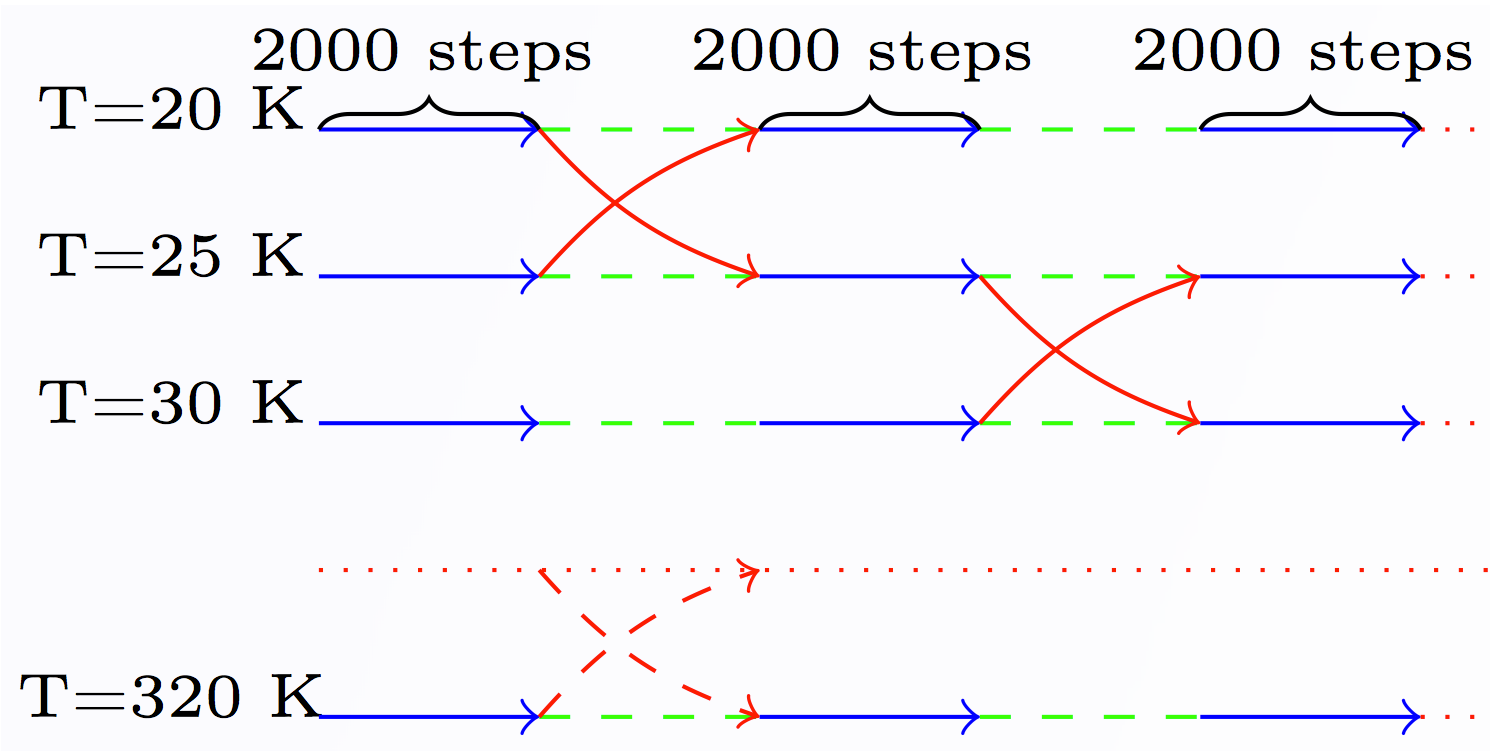
\includegraphics[width=12cm]{ptmd.png}
\end{center}
\caption{Schematic representation of the PTMD algorithm used to explore PES. In this example, it consists of 64 replicas with
temperatures going from 20 to 320~K by steps of 5~K. Every 2000 MD step, exchanges are tested using a Metropolis criterion between
simulations corresponding to adjacent temperatures. Some tests are successful (plain red arrows) which lead to exchanges of configurations
while others are unsuccessful (dashed red arrows). This scheme corresponds to a synchronized version of the PTMD algorithm although
non-synchronized versions also exist that are computationally more efficient when the number of replicas increases \cite{Bussi2008c}. JC autres ref a mettre Gallichio QUELQUECHOSE }
\label{ptmd}
\end{figure}

In addition to its use in the context of global optimization, one can also extract from PTMD simulations properties at different temperatures,
for instance, densities of states. The latter can be used to directly compute heat capacities as a function of the simulated temperatures.
Alternatively, one can use the multiple histogram method \cite{Labastie1990} which takes advantage from the fact that the densities of
states at the different temperatures overlap to reduce the noise in the computed heat capacities and derive values for temperatures between
the  simulated ones.
  
\section{Applications} \label{appl}

\subsection{Isolated water clusters}  \label{bare_water}
%	- structural and energetic properties : 
%	- IR ?
%	- Thermodynamical properties (i.e tres court)
As mentioned in previous section, describing the weak intermolecular interactions within water clusters with SCC-DFTB  requires a delicate description of the balance between long range interactions, namely hydrogen bonds, Coulomb interactions between distant charge fluctuations, London dispersion, polarization and Pauli repulsion. A pre-requisite
for the validity of the SCC-DFTB potential energy surface
for water clusters is a correct description of the H$_2$O-H$_2$O interaction.  This was achieved via the CM3 charge correction and the inclusion of a dispersion  term in the initially implemented SCC-DFTB hamiltonian \cite{SimonPCCP2012}. We obtained a water-water interaction energy of 3.08 kcal.mol$^{-1}$, in agreement with experimental results (3.16$\pm$0.03 kcal.mol$^{-1}$ \cite{Rocher2011}). However, the dipole moment of the water molecule was found to be overestimated with respect to the experimental value ( 2.04\,D vs 1.85\,D \cite{Dyke1973}). Using both these CM3 and dispersion corrections, we obtained the correct energy order for the structural isomers of the water hexamer (H$_2$O)$_6$ (see geometries and relative energies in Figure \ref{fig:geoms_w6}) with respect to CCSD(T) calculations in the complete basis set (CBS)  limit \cite{SimonJCP2013}. The CCSD(T)/CBS dissociation energy ((H$_2$O)$_n$ $\rightarrow$ nH$_2$O) was also reproduced for a variety of isomers of (H$_2$O)$_n$, (n=2-10) (see Figure~\ref{fig:nrj_wn}).
	
	 \begin{figure}[!ht]
	  \begin{center}
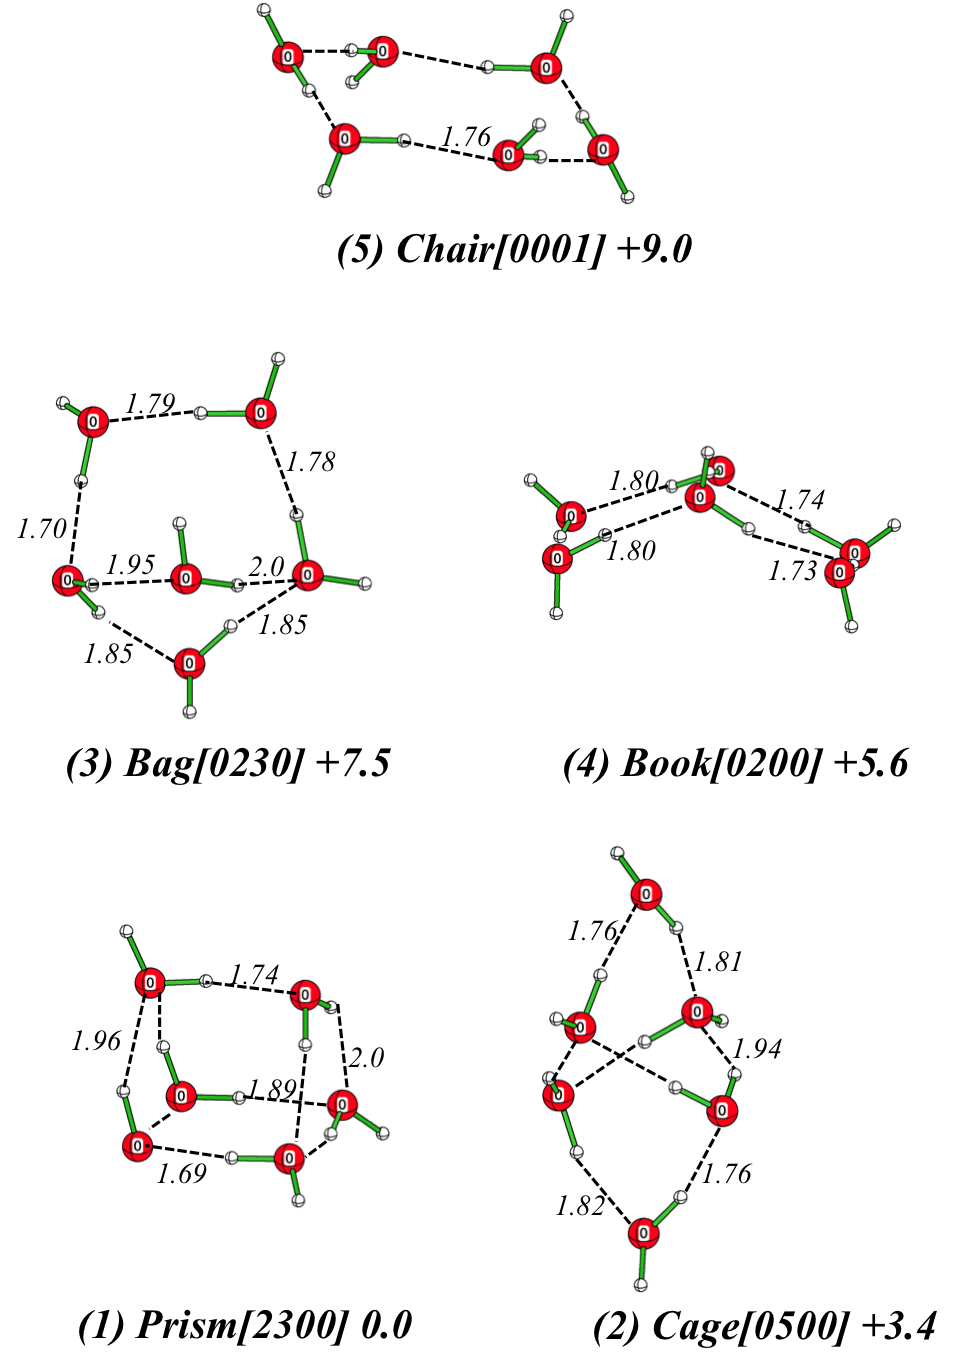
\includegraphics[width=10cm]{geoms_w6.png}
  \end{center}
\caption{Optimized geometries of the isomers of (H$_2$O)$_6$ determined at the SCC-DFTB level using CM3 charges and dispersion corrections. The relative energies (in kJ.mol$^{-1}$) with respect to the most stable (Prism) isomer are also reported. The [mnop] nomenclature means that the water molecules within the cluster are organized within cycles among which m are constituted of three molecules and n,o and p cycles  of four, five and six molecules respectively.  }
\label{fig:geoms_w6}
\end{figure}

	
			 \begin{figure}[!ht]
		  \begin{center}
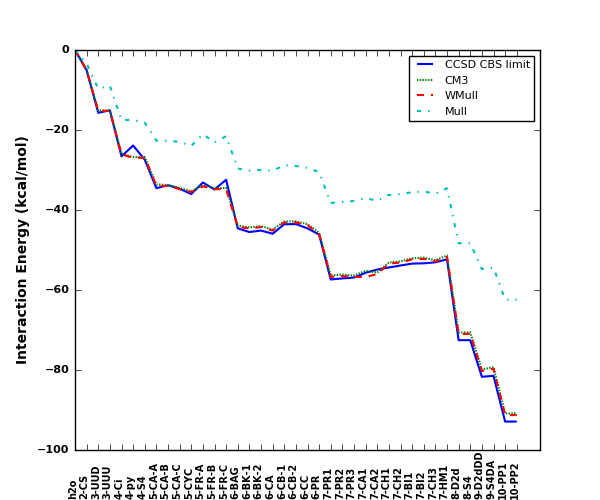
\includegraphics[width=14cm]{ener_Wn1.png}
  \end{center}
\caption{Interaction energies within water clusters : comparison between wavefunction results (CCSD-CBS limit) \cite{bench_nrj_Wn_JPCA2011} and SCC-DFTB values using CM3 charges (DOH=0.13)\cite{SimonPCCP2012},  WMull charges ($t_{OH}$=0.39, see \cite{Michoulier18b}), and Mulliken charges. The x-axis represents water clusters of increasing size, under different isomeric forms using the acronyms of ref.  \cite{bench_nrj_Wn_JPCA2011} }
\label{fig:nrj_wn}
\end{figure}


		We also  more recently determined  Weighted Mulliken charges for water clusters \cite{Michoulier18b} as an alternative to CM3 charges because, as mentioned in section 1, Weighted Mulliken charges  charges are more convenient for the study of large systems (implementation and computational cost), which is one of our perspectives . We found a t$_{OH}$ parameter that was able to reproduce the results obtained with CM3 charges maintaining the dispersion term (see Figure 1). This will be used for the study of the description of water ice and liquid water (see section 3.5).
				
		Using the adjusted SCC-DFTB potential, conformational dynamics were investigated for (H$_2$O)$_6$ \cite{SimonJCP2013}  and (H$_2$O)$_8$ \cite{SimonCOMP2013}, followed by a more quantitative study based on PTMD simulations in order to determine heat capacities \cite{Oliveira2015}. These two clusters can be distinguished by their density of low energy isomers :  regarding (H$_2$O)$_6$ , the "Prism" isomer is the most stable, closely followed by the Cage,  Bag,  Book and Chair isomers within an energy range of 9 kJ.mol$^{-1}$ (see Figure \ref{fig:geoms_w6}). On the opposite, "Cubic" isomers constitute the only pool of low energy isomers  for (H$_2$O)$_8$, the first non cubic structure being located at about 20 kJ.mol$^{-1}$ above  (see for instance Fig. 3 in ref. \cite{SimonCOMP2013}).  As a consequence, the melting of (H$_2$O)$_6$ was found to occur at $\sim$ 80\,K (pronounced peak in the heat capacity curve) while that of (H$_2$O)$_8$ was  found at a much higher temperature ($\sim$ 180\,K \cite{Oliveira2015}).  We may note that similar studies - via PTMC simulations-  were achieved by Choi \cite{Choi2012} using a SCC-DFTB hamiltonian plus dispersion interactions, and also a corrected version of this hamiltonian including both H-bonds and third order corrections. He found  melting temperatures of 134 K and 210 K respectively using the two approaches, illustrating the sensitivity of the results to the description of the PES.    %\red{Il reste une ref de Mathias a mettre dans la partie bare clusters
%\ Simulation of the (H2O)8 cluster with the SCC-DFTB electronic structure method}

		
		
		The evolution of the IR spectra of water clusters as a function of internal energy were also studied  \cite{SimonPCCP2012, SimonJCP2013, SimonCOMP2013}, but the objective was to compare with the results for water clusters adsorbed on PAHs, that are described in section 3.3. %. The two latter studies were performed in order to compare the results with those obtained for water clusters adsorbed on PAHs, that will be described in section 3.3.\\% but more for comparison with the water cluster adsorbed on the PAH surface. \\
	
%The relative energies of the water hexamers isomers were found to be comparable to CCSD(T) values \cite{SimonJCP2013}. %We note the using CM3 charges instead of Mulliken ones did not lead to much geometry changes, which compare nicely to wavefunction ones. 

%\\
%Other works : DFTB3 + others ? 

\subsection{Water clusters in interaction with neutral of ionic molecules}

Taking advantage of the SCC-DFTB parametrization transferability, its applications were further extended 
from bare water clusters to aggregates containing both water molecules and an additional species, either
neutral or ionic. In particular, protonated water clusters have been the subject of several studies and used
as test cases for the validation of the SCC-DFTB approach in describing hydrogen-bonded systems \cite{Yu2007,Goyal2011,Dominguez2015}.
Over the last years, our group has also devoted significant efforts to extend the applicability of the
SCC-DFTB approach to investigate aggregates of atmospheric and astrophysical interest. Three main studies
were devoted to:  (i) the thermodynamical properties of protonated water clusters \cite{Korchagina2017} ; (ii)
the structure of sulfate-containing water clusters \cite{Korchagina2016} ; (iii) the reactivity of H with CO adsorbed on water clusters \cite{Korchagina2017a}.
We now briefly review these three studies in order to highlight the performances of SCC-DFTB in describing
water aggregates containing an impurity.


\subsubsection{Protonated water clusters} 

This first study was motivated by recent experimental results by Boulon~\textit{et al.}
\cite{Boulon2014}  who measured the heat capacity curves of protonated water clusters (H$_{2}$O)$_{n}$H$^{+}$ with $n$ going
from 20 to 118. Transition temperatures were then extracted from those curves and compared to each other. For $n$ up to $\sim$45,
transition temperatures vary very roughly as a function of $n$ with sharp variations between consecutive sizes. This behavior is
characteristic of various properties in small aggregates, molecular or atomic \cite{Jortner1992,Labastie_book}. For larger species,
the evolution becomes more monotonous. Even more interesting is the presence of  clusters displaying a notably high transition
temperature with respect to surrounding sizes. This is the case of  (H$_{2}$O)$_{21}$H$^{+}$, (H$_{2}$O)$_{28}$H$^{+}$ and
(H$_{2}$O)$_{55}$H$^{+}$. Although the latter case is more contentious \cite{Hansen2009}, previous studies have already highlighted
the "magic size" character of those three specific aggregates \cite{Lee1998,Shin2004,Wu2005,Hansen2009}. In particular,
(H$_{2}$O)$_{21}$H$^{+}$ has been the subject of numerous theoretical and experimental studies \cite{Hodges2000,Wu2005,Iyengar2005,Miyazaki2004,Shin2004,Singh2006}.

Using the SCC-DFTB approach in combination with the parallel-tempering molecular dynamics (PTMD) algorithm, we
intended to explain the higher transition temperature of (H$_{2}$O)$_{21}$H$^{+}$ as compared to adjacent sizes
\cite{Korchagina2017}. To do so, we first modelled the heat capacity curves for the (H$_{2}$O)$_{20-23}$H$^{+}$
clusters and compared them to the experimental data of  Boulon \textit{et al.} (see Figure~\ref{capa} (a)). The theoretical
curves presented in Figure~\ref{capa} (b) were obtained using the same SCC-DFTB potential developed by Simon \textit{et al.}
to describe bare water clusters \cite{SimonPCCP2012,SimonJCP2013} and discussed in section~\ref{bare_water}. The
good agreement between the experimental and theoretical curves was a proof of the accuracy of this parametrization
to describe the thermodynamical properties of protonated water clusters. To go a step further into the interpretation of
the experimental data, we analysed the PTMD simulations in terms of various structural and dynamical indicators and looked
at their evolution as a function of the temperature: number and size of water molecule rings, distribution of angles in the whole
cluster or restricted to the first solvation shell of each water molecule, localization of the excess proton and correlation functions
to characterize the dynamics of the aggregates. All structural and dynamical indicators highlighted the peculiar character of 
(H$_{2}$O)$_{21}$H$^{+}$. For instance, the transition from a low-temperature structure made of 100\% five-membered rings
(which is characteristic of the distorted pentagonal dodecahedron (5$^{12}$) structure of the lowest-energy isomer of
(H$_{2}$O)$_{21}$H$^{+}$ presented in Figure~\ref{h2o21} \cite{Hodges2000,Wu2005,Iyengar2005,Miyazaki2004,Shin2004,Singh2006})
to liquid-like structures is abrupt and takes place over a very narrow range of temperatures. In contrast, the transition is much
smoother in (H$_{2}$O)$_{20}$H$^{+}$ and even monotonous in (H$_{2}$O)$_{22}$H$^{+}$. This difference between an
abrupt transition in (H$_{2}$O)$_{21}$H$^{+}$ against a smooth one in the other aggregates was also observed for the other
structural indicators and is responsible for the steepness of the (H$_{2}$O)$_{21}$H$^{+}$ caloric curve. In addition,
taking advantage of  the ability of the SCC-DFTB approach to describe bond breaking and forming, the temperature dependence
of proton-transfer frequency was also evaluated in the four clusters. For (H$_{2}$O)$_{20}$H$^{+}$ and (H$_{2}$O)$_{21}$H$^{+}$,
which are characterized by a crystal-like structure at low temperature, proton hops occur only a few Kelvin above the transition
temperature and their frequency continuously increases from that point. In contrast, in (H$_{2}$O)$_{22}$H$^{+}$ and
(H$_{2}$O)$_{23}$H$^{+}$, which display a more liquid-like structure at low temperature, proton hops exist below the
transition temperature resulting from the difficulty of less organized structures to accommodate the excess proton.

From a technical point of view, PTMD simulations could not safely be used to obtain proton-transfer frequency in a non-biased way.
Consequently, it was achieved for each cluster by propagating ten micro-canonical trajectories per temperature using initial conditions
randomly extracted from the PTMD simulations. Each micro-canonical simulation was 200~ps long which allowed to extract converged
and meaningful dynamical informations from their analysis. Such study was made possible by both the computational efficiency of the
SCC-DFTB formalism, its ability to describe bond breaking and bond forming, and the transferability of the SCC-DFTB parametrization.
Of course, a properly parametrized force field could also have been applied to conduct this study. Nevertheless, finding a suitable force
field to calculate heat capacity curves has been shown to be difficult in bare water clusters \cite{Pedulla1998,Douady2009} and is probably
even more touchy for protonated ones. Furthermore, the study by Korchagina \textit{et al.} represents a step further in the validation of
SCC-DFTB to describe water clusters and can be used as basis to further extend its parametrization to include other species such as sulfates.


\begin{figure}
\begin{center}
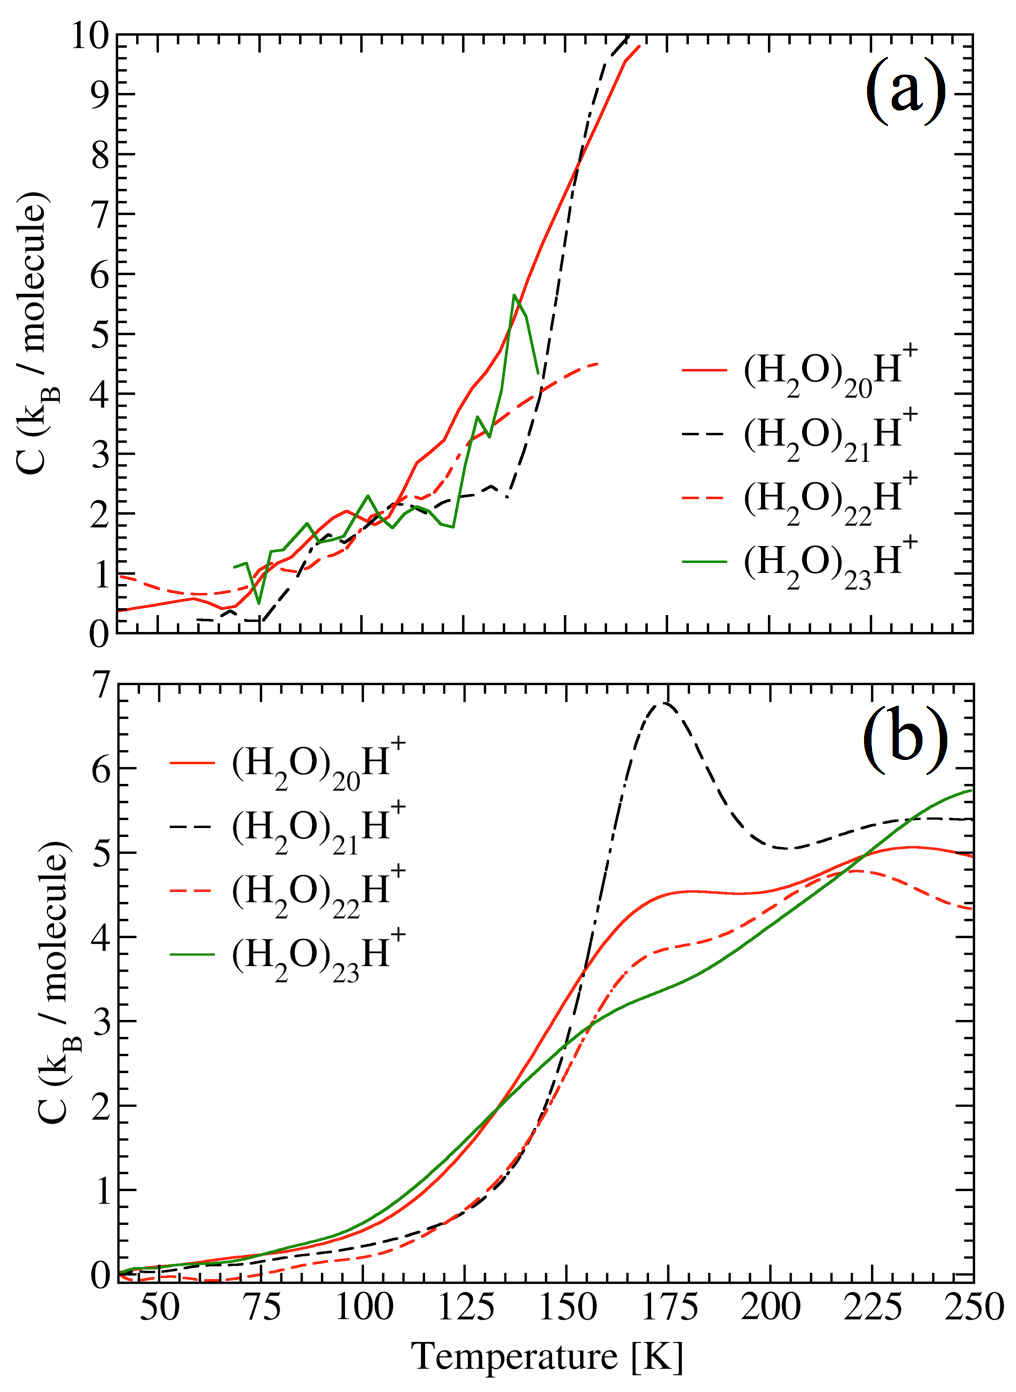
\includegraphics[width=8cm]{Capa.png}
\end{center}
\caption{(a) Experimental and (b) theoretical heat capacity curves of (H$_{2}$O)$_{20-23}$H$^{+}$ clusters plotted as a function of temperature.
Adapted from \cite{Korchagina2017} with permission of The Royal Society of Chemistry (http://dx.doi.org/10.1039/C7CP04863G).}
\label{capa}
\end{figure}

\begin{figure}
\begin{center}
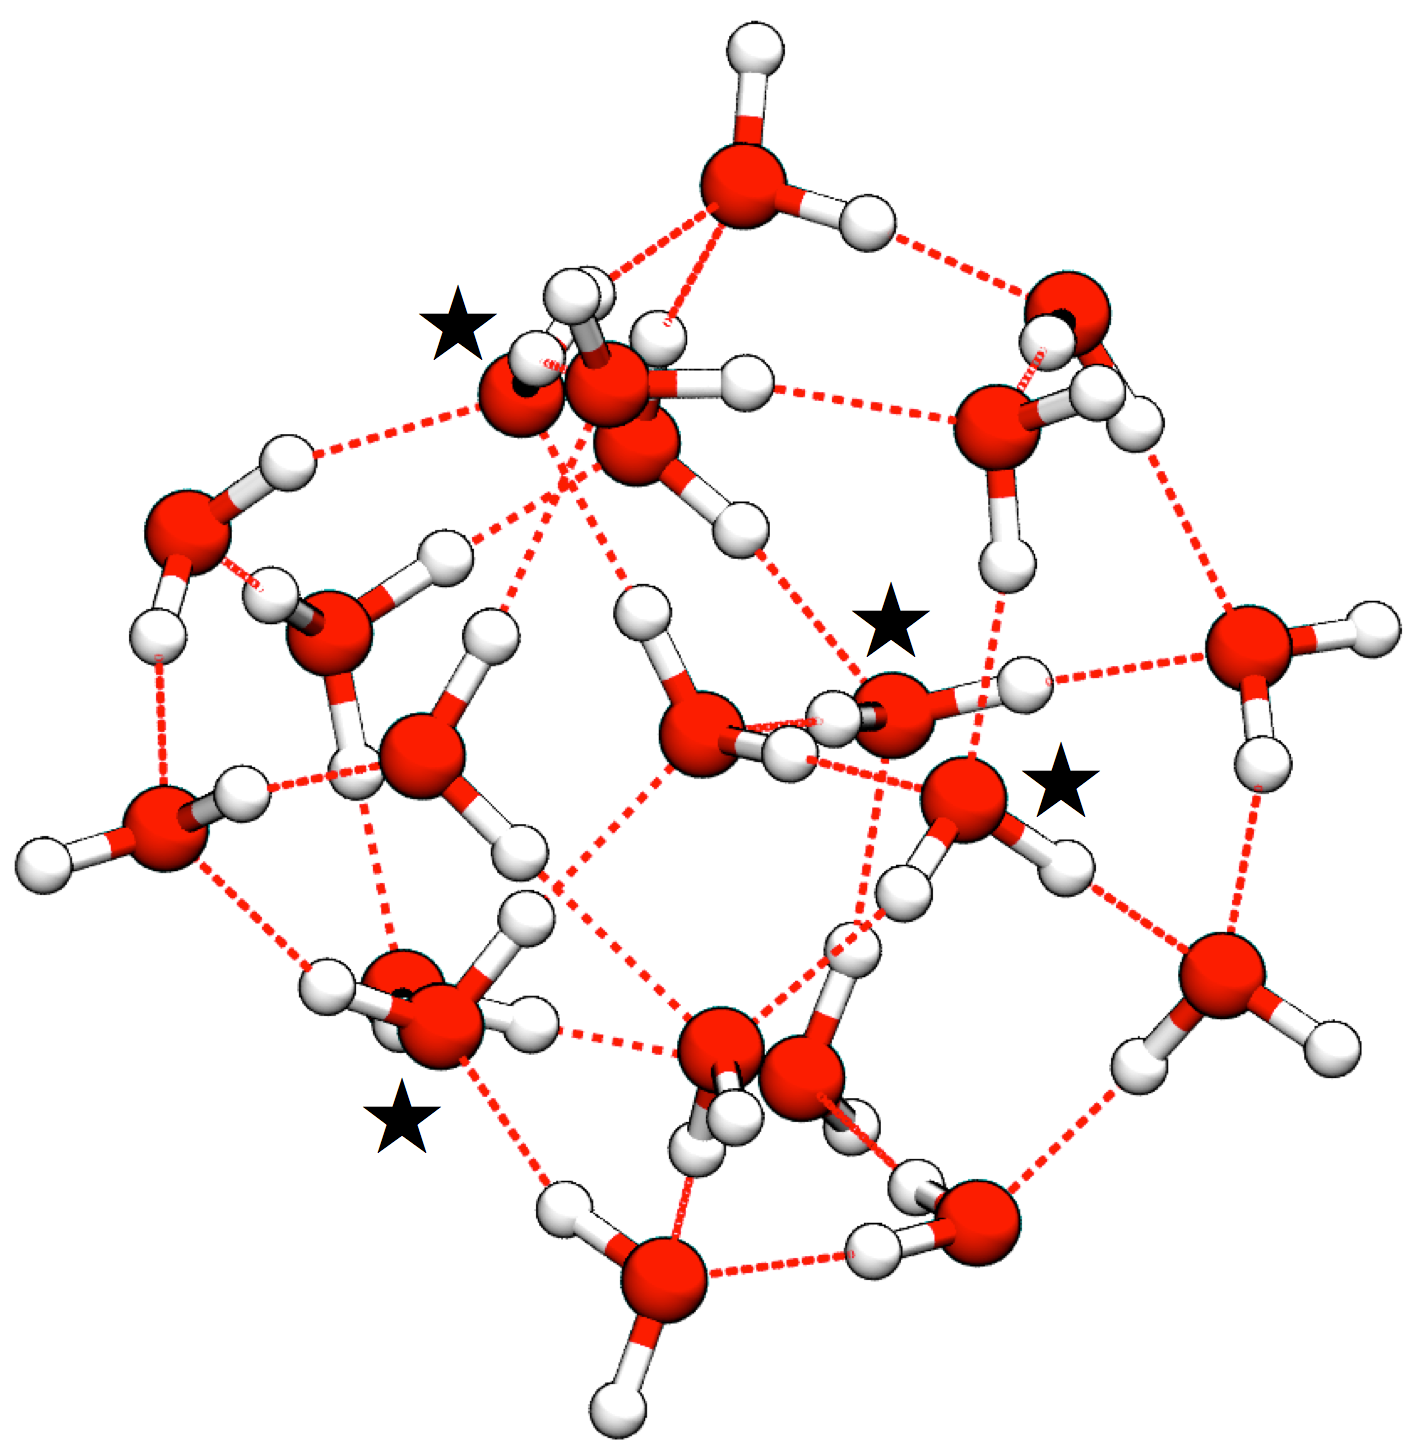
\includegraphics[width=5cm]{H2O21.png}
\end{center}
\caption{Lowest-energy isomer of (H$_{2}$O)$_{21}$H$^{+}$. The $\star$ symbol denotes the four
water molecules of the outer sphere hydrogen-bonded to the central water molecule.}
\label{h2o21}
\end{figure}

\subsubsection{Sulfate-containing water clusters} 

Sulfuric acid (H$_{2}$SO$_{4}$), sulfate ion (SO$_{4}^{2-}$) as well as other ions such as
nitrate or ammonium are important components of the lower layers of the atmosphere as they play a key role
in facilitating nucleation, ion-ion recombination, and growth of particles which lead to the formation of aerosol layers \cite{yu,shaw,kulmala,yu2,Metzger2010,Schobesberger2013,Kurten2014,Dunne2016,Lehtipalo2016, Boyer2017}.
As an accurate understanding of this latter process is still missing, a number of studies have been conducted
to highlight the specific role of each aforementioned chemical species.
In particular, various sulfate-containing water aggregates have been characterized experimentally \cite{wang2,Wang2001,Zhou2006,Bush2007,brein1,brein2,yang1,wang1}. Theoretical calculations have also been
conducted to explore the potential energy surface (PES) of (H$_{2}$O)$_{n}$SO$_{4}^{2-}$ (n=1--50) \cite{Zhou2006,brein1,brein2,pye1,whitehead,wong1,wang1,ohanessian,lambrecht1,wan,mardirossian,Smeeton2015,Hey2016} 
and (H$_{2}$O)$_{n}$H$_{2}$SO$_{4}$ (n=1--9) \cite{bandy1,arstila1,re1,ding2003,ding2004,miller3,miller2} aggregates using
methodologies based on: (i) DFT or wavefunction optimization of structures constructed from chemical intuition or previously
reported in the literature ; (ii) extensive exploration of the PES with a non-polarisable rigid force field ; (iii) pre-screening of structures
with a force  field combined to subsequent geometry optimizations with a higher level approach (DFT or wavefunction). Although
highly valuable in terms of structural information, those approaches are limited when it comes to dynamical studies taking into 
account finite temperature effects.

So, in order to develop a scheme that can model both (H$_{2}$O)$_{n}$SO$_{4}^{2-}$ and (H$_{2}$O)$_{n}$H$_{2}$SO$_{4}$
aggregates in a consistent way and that is efficient enough to perform extensive simulations for species containing up to
$\sim$20-30 water molecules, we recently proposed a SCC-DFTB parametrization for sulfate-containing water aggregates \cite{Korchagina2016}.
The potential is based on the aforementioned parametrization for water and includes the sulfur-hydrogen and sulfur-oxygen
integrals and repulsive potential included in the mio-set of Slater-Koster tables \cite{elstner98,Niehaus2001}. To properly
describe both sulfate ion and sulfuric acid we used a D$_{OS}$ parameter of 0.238 for the definition of the CM3 charges.
The D$_{SH}$ parameter was set to zero.

This potential was validated for a variety of species:  (H$_{2}$O)$_{n}$SO$_{4}^{2-}$ ($n$ = 1-6, 10, 12, 13, 15, 20) and
(H$_{2}$O)$_{n}$H$_{2}$SO$_{4}$ ($n$ = 1-6, 10, 15, 20). In each case, extensive PTMD simulations were performed
complemented by a large number of geometry optimizations to determine the low-energy isomers of each species at the 
SCC-DFTB level. The structures were compared to the literature for sizes up to $n$ = 6 and 13 for (H$_{2}$O)$_{n}$H$_{2}$SO$_{4}$
and  (H$_{2}$O)$_{n}$SO$_{4}^{2-}$, respectively. The SCC-DFTB isomers were in good agreement with structures obtained
at the DFT or wavefunction levels of theory. Indeed, for small clusters, the SCC-DFTB simulations located most of the isomers
previously reported in the literature and also found some new ones. In the case of (H$_{2}$O)$_{n}$H$_{2}$SO$_{4}$ aggregates,
SCC-DFTB located ionic (\textit{i.e.} deprotonated) structures at rather low relative energy. However, in contrast to previously
reported structures at the DFT level \cite{re1,ding2004}, they are not the lowest-energy isomer. At the DFT level, this
question is very sensitive to computational details such as functional or basis-set extension, which mitigates the discrepancy
between DFT and SCC-DFTB results. From an energetics point of
view, considering 12 isomers of the (H$_{2}$O)$_{1-4}$SO$_{4}^{2-}$ aggregates, SCC-DFTB binding energies display a mean
absolute error (MAE) of 1.38~kcal.mol$^{-1}$ as compared to B3LYP/QZVP results (a maximum error of 2.13~kcal.mol$^{-1}$ was
obtained). Similar results were also obtained for  (H$_{2}$O)$_{n}$H$_{2}$SO$_{4}$ clusters. For (H$_{2}$O)$_{12}$SO$_{4}^{2-}$ and
(H$_{2}$O)$_{13}$SO$_{4}^{2-}$, which have been extensively studied at the DFT level by Thaunay \textit{et al. }\cite{ohanessian},
SCC-DFTB performs also quite well as it located a number of the previously reported structures. For the largest size considered,
\textit{i.e.} $n$ = 20, we were the first to report low-energy isomers for (H$_{2}$O)$_{20}$SO$_{4}^{2-}$ and (H$_{2}$O)$_{20}$H$_{2}$SO$_{4}$
using an \textit{ab initio} exploration of the PES. Interestingly, all the SCC-DFTB low-energy structures of (H$_{2}$O)$_{20}$SO$_{4}^{2-}$
display no dangling hydrogen bond (see Figure~\ref{large_soufre} (a) for the lowest-energy isomer). This is in agreement with infrared
spectroscopic measurements performed by O'Brien \textit{et al.} \cite{brein1} and gives further credit to the accuracy of the
SCC-DFTB approach to describe those aggregates. In contrast, we also demonstrated that (H$_{2}$O)$_{n}$H$_{2}$SO$_{4}$
clusters are always characterised by dangling hydrogen atoms, either for the small and large sizes (see Figure~\ref{large_soufre} (b)
for the lowest-energy isomer of (H$_{2}$O)$_{20}$H$_{2}$SO$_{4}$). This important difference in structure between
(H$_{2}$O)$_{20}$SO$_{4}^{2-}$ and (H$_{2}$O)$_{20}$H$_{2}$SO$_{4}$ would probably lead to significant differences in
thermodynamical behavior as could be highlighted in their heat capacity curves. This question is actually under study.

\begin{figure}
\begin{center}
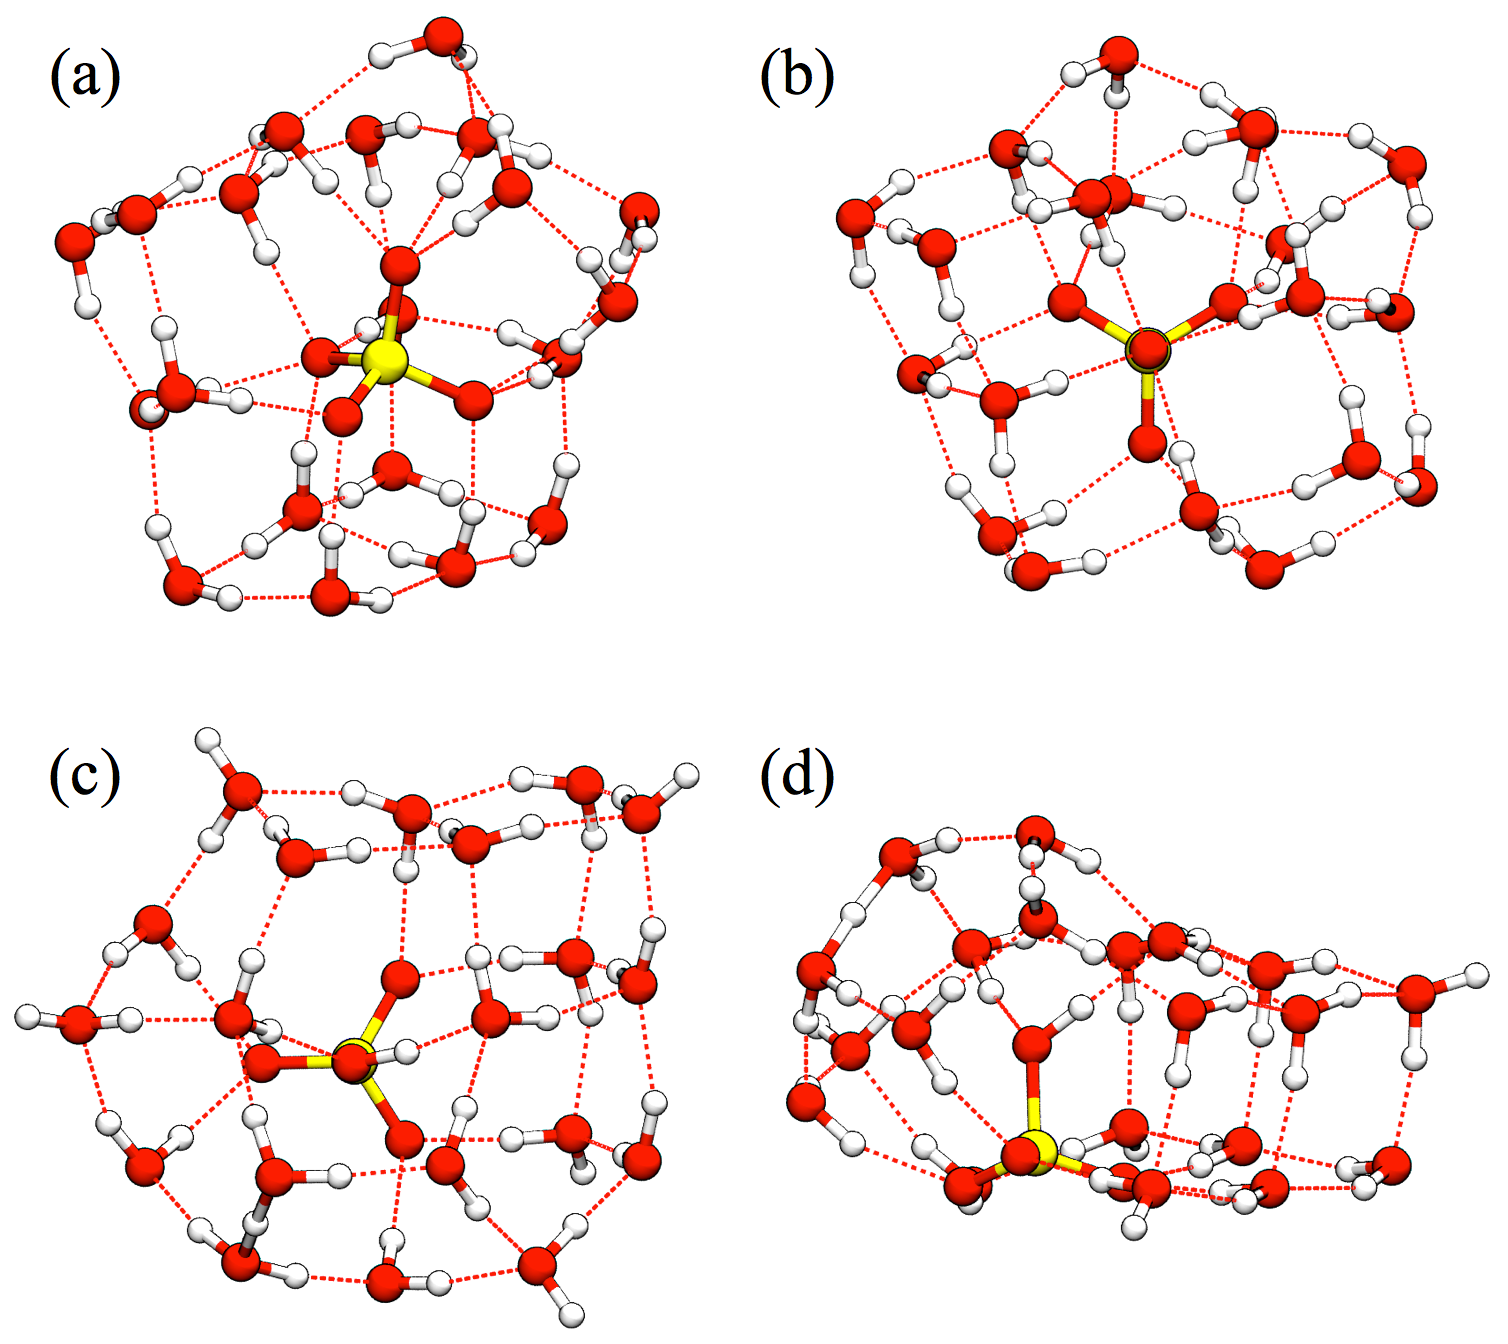
\includegraphics[width=8cm]{sulfate.png}
\end{center}
\caption{Lowest-energy isomer of   (H$_{2}$O)$_{20}$SO$_{4}^{2-}$ (a,b) and (H$_{2}$O)$_{20}$H$_{2}$SO$_{4}$ (c,d) (without considering
zero-point energy) determined through a SCC-DFTB exploration of the potential energy surface. Two different views are displayed for each isomer.}
\label{large_soufre}
\end{figure}

Ammoniac and some organic molecules such as dimethylamine have been shown to interact with sulfuric acid in
the atmosphere which strongly impacts the formation of aerosols \cite{Metzger2010,Schobesberger2013,Kurten2014,Lehtipalo2016}.
Consequently, in order to model phenomena of atmospheric interest, further parametrization of the SCC-DFTB potential will
be necessary to describe those species, in addition to water and sulfuric acid. This is an ongoing work in our group
as we are now developing and validating a SCC-DFTB potential for ammonium (NH$_{4}^{+}$) and ammoniac (NH$_{3}$).
In contrast to  SO$_{4}^{2-}$ and H$_{2}$SO$_{4}$, a difficulty arises resulting from the description of sp$^{3}$ hybridized
nitrogen atoms. Indeed, it has been highlighted in several studies that the actual parametrization of DFTB3 does not
correctly describe the proton affinity of sp$^{3}$ hybridized nitrogen \cite{Gaus2011,Gaus2013,Gaus2014}. This is
related to the parametrization of the Slater-Koster integrals and is also true for SCC-DFTB calculations. Indeed, in
H$_{2}$O-NH$_{4}^{+}$, the original SCC-DFTB  parametrization leads to a N-H distance (H-bonded to H$_{2}$O) of
1.14~\AA~against 1.03~\AA~at the MP2/Def2TZVP level \cite{Weigend2005,Weigend2006}. This effect worsens when the
number of water molecules increases. We have now proposed a new parametrization of the N-H Slater-Koster table
especially optimized  to describe NH$_{4}^{+}$ and NH$_{3}$ interacting with water molecules. It leads to the correct
 lowest-energy structures of the (H$_{2}$O)$_{1-4}$NH$_{4}^{+}$ aggregates (see Figure~\ref{ammonium}) and
 binding energies in good agreement with MP2/Def2TZVP calculations.

\begin{figure}
\begin{center}
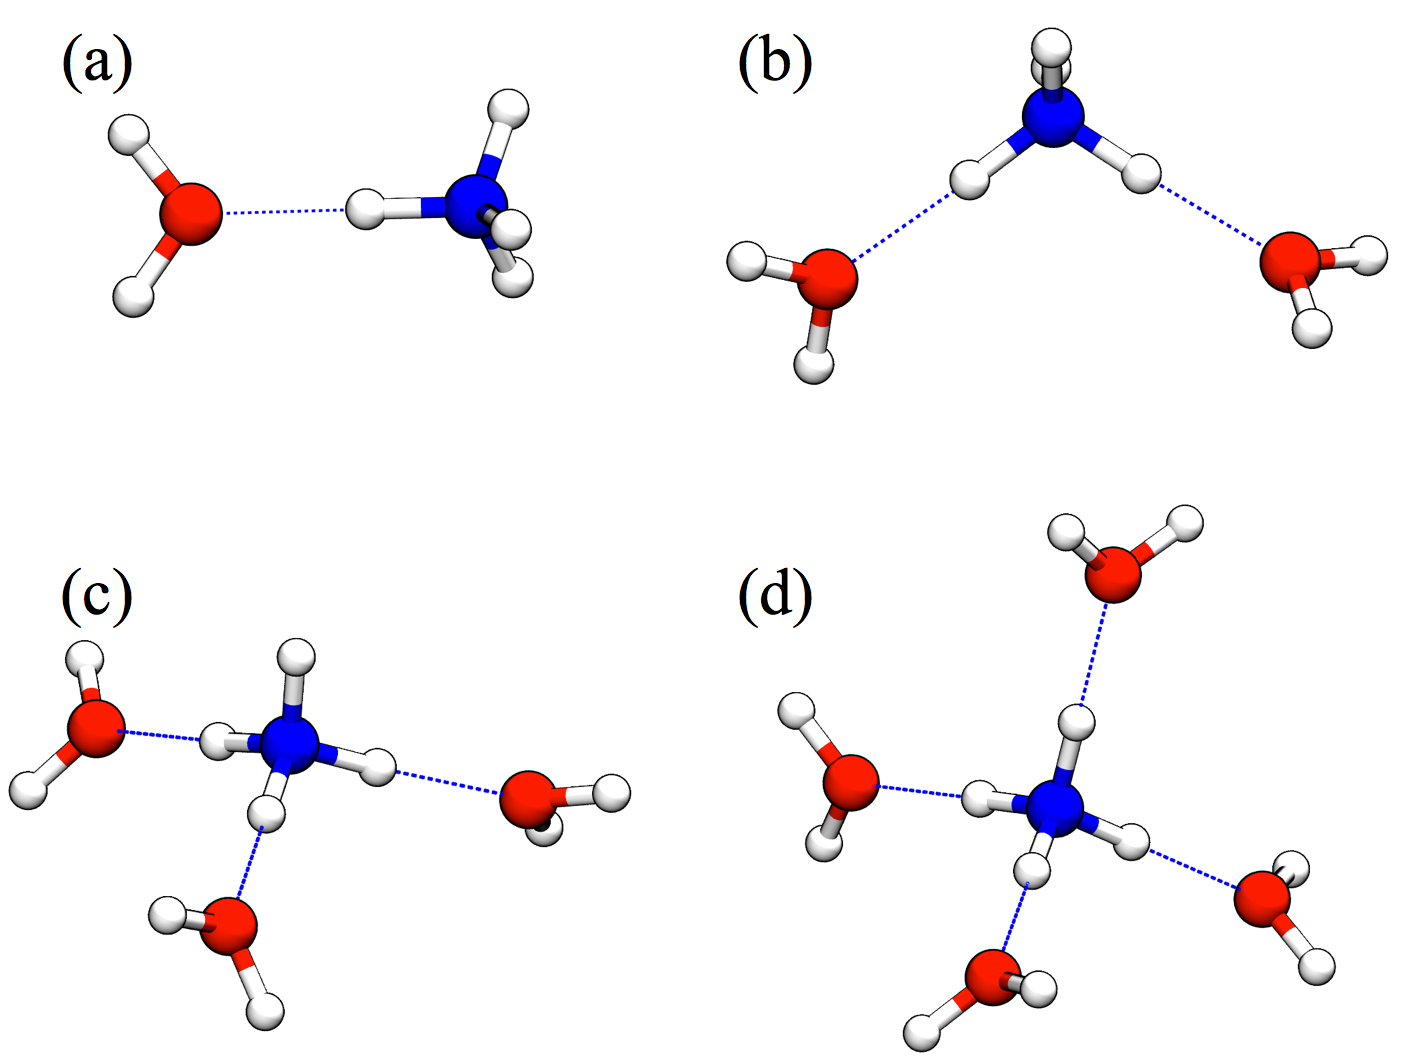
\includegraphics[width=8cm]{ammonium.png}
\end{center}
\caption{Lowest-energy isomers of (a)  (H$_{2}$O)NH$_{4}^{+}$, (b) (H$_{2}$O)$_{2}$NH$_{4}^{+}$, (c) 
(H$_{2}$O)$_{3}$NH$_{4}^{+}$, and (d) (H$_{2}$O)$_{4}$NH$_{4}^{+}$ determined through a SCC-DFTB
exploration of the PES with optimised parametrization.}
\label{ammonium}
\end{figure}

\subsubsection{Reactivity of H with CO on water clusters}  \label{reactivity}

A third study was conducted to  describe the reactivity of H with CO 
adsorbed on water clusters of various sizes, (H$_{2}$O)$_{n}$ with $n$ = 0-10. This reaction is of fundamental interest
as it represents the first step of a general mechanism leading to the formation of complex oxygenated species present
in the interstellar medium (ISM) \cite{book1,tielens1,crovisier1,watanabe2,watanabe3,hidaka1}. Consequently, several
experimental \cite{hiraoka1,hiraoka2,pirim1,watanabe1,watanabe2} and theoretical \cite{woon1,cao1,woon2,rimola1,peters1}
studies have been performed to describe it, in particular, to highlight the role of supporting water molecules in facilitating
the reaction. Most of the theoretical works devoted to this question were performed using a static picture and focused
on the relative energies of reactants, products and transition states. They were performed using highly accurate
methods such as restricted coupled cluster RCCSD(T) or Davidson-corrected internally contracted MRCI+Q.

To complement those studies and provide a dynamical picture of the H + CO(H$_{2}$O)$_{n}$ $\rightarrow$ HCO(H$_{2}$O)$_{n}$
reaction, we performed a SCC-DFTB study focusing on the reactivity induced by a direct collision of an H atom with
the CO(H$_{2}$O)$_{n}$ cluster \cite{Korchagina2017a}.  As for the description of proton transfers in (H$_{2}$O)$_{n}$H$^{+}$
(see above), this study was made possible by the SCC-DFTB ability  to describe bond breaking and bond
forming. In a first step, we evaluated the accuracy of SCC-DFTB to describe the PES of the systems of interest. To do so,
we determined the binding energies within the CO(H$_{2}$O)$_{n}$ and HCO(H$_{2}$O)$_{n}$ systems as well as to the HCO
formation energies. The SCC-DFTB results were found in good agreement with DFT (using the B3LYP-D3 and B97D functional)
and MP2 methods, which validated the use of SCC-DFTB for this study. Given the small energies characteristic of the
interaction of CO and HCO with water clusters, this is already a very encouraging achievement to be able to qualitatively
reproduce them at the SCC-DFTB level. In a second step, the reaction was studied in the following manner: (i) for each size $n$,
a CO(H$_{2}$O)$_{n}$ aggregate was equilibrated at 70~K ; (ii) 3392 (2000 for CO(H$_{2}$O)$_{10}$) initial conditions
(positions and velocities) were extracted from the equilibration dynamics to initialize the collision trajectories ; (iii)
3392 (2000 for CO(H$_{2}$O)$_{10}$)  micro-canonical collision trajectories were conducted of 10~ps each ; (iv) all
trajectories were analysed in terms of successful reaction and collisional pathway to provide statistically converged
information describing the reaction. 

The analysis of those data demonstrated that the size of the water cluster has a strong influence on the reaction.
Indeed, for CO(H$_{2}$O), although the transient formation of HCO is possible, the unique water molecule is not
able to dissipate the excess kinetic energy transferred from H to CO. This leads to the re-dissociation of HCO in 63.2\%
of trajectories and only 3.1\% of successful formation of HCO. For CO(H$_{2}$O)$_{2}$ and CO(H$_{2}$O)$_{3}$, the energy
dissipation is effective enough to allow for the stable formation of HCO although it dissociates from the water cluster in
58.1 and 50.9\% of cases, respectively. Of course, this is a bad point for further hydrogenation of HCO and the formation
of complex oxygenated molecules. From CO(H$_{2}$O)$_{4}$, the formation of a stable HCO molecule attached to the water
cluster is the predominant pathway with more than 50\% of occurrence. Finally, for CO(H$_{2}$O)$_{10}$, this number 
decreases in favor of trajectories were H and CO do not collide. This is explained by the larger surface area of (H$_{2}$O)$_{10}$
with respect to smaller clusters. The successful formation of HCO, either bound to the water molecules or not, can be summarized
in Figure~\ref{recomb} that represents the reaction cross section $\Omega$ for the HCO formation as a function of the water
cluster size.

\begin{figure}
\begin{center}
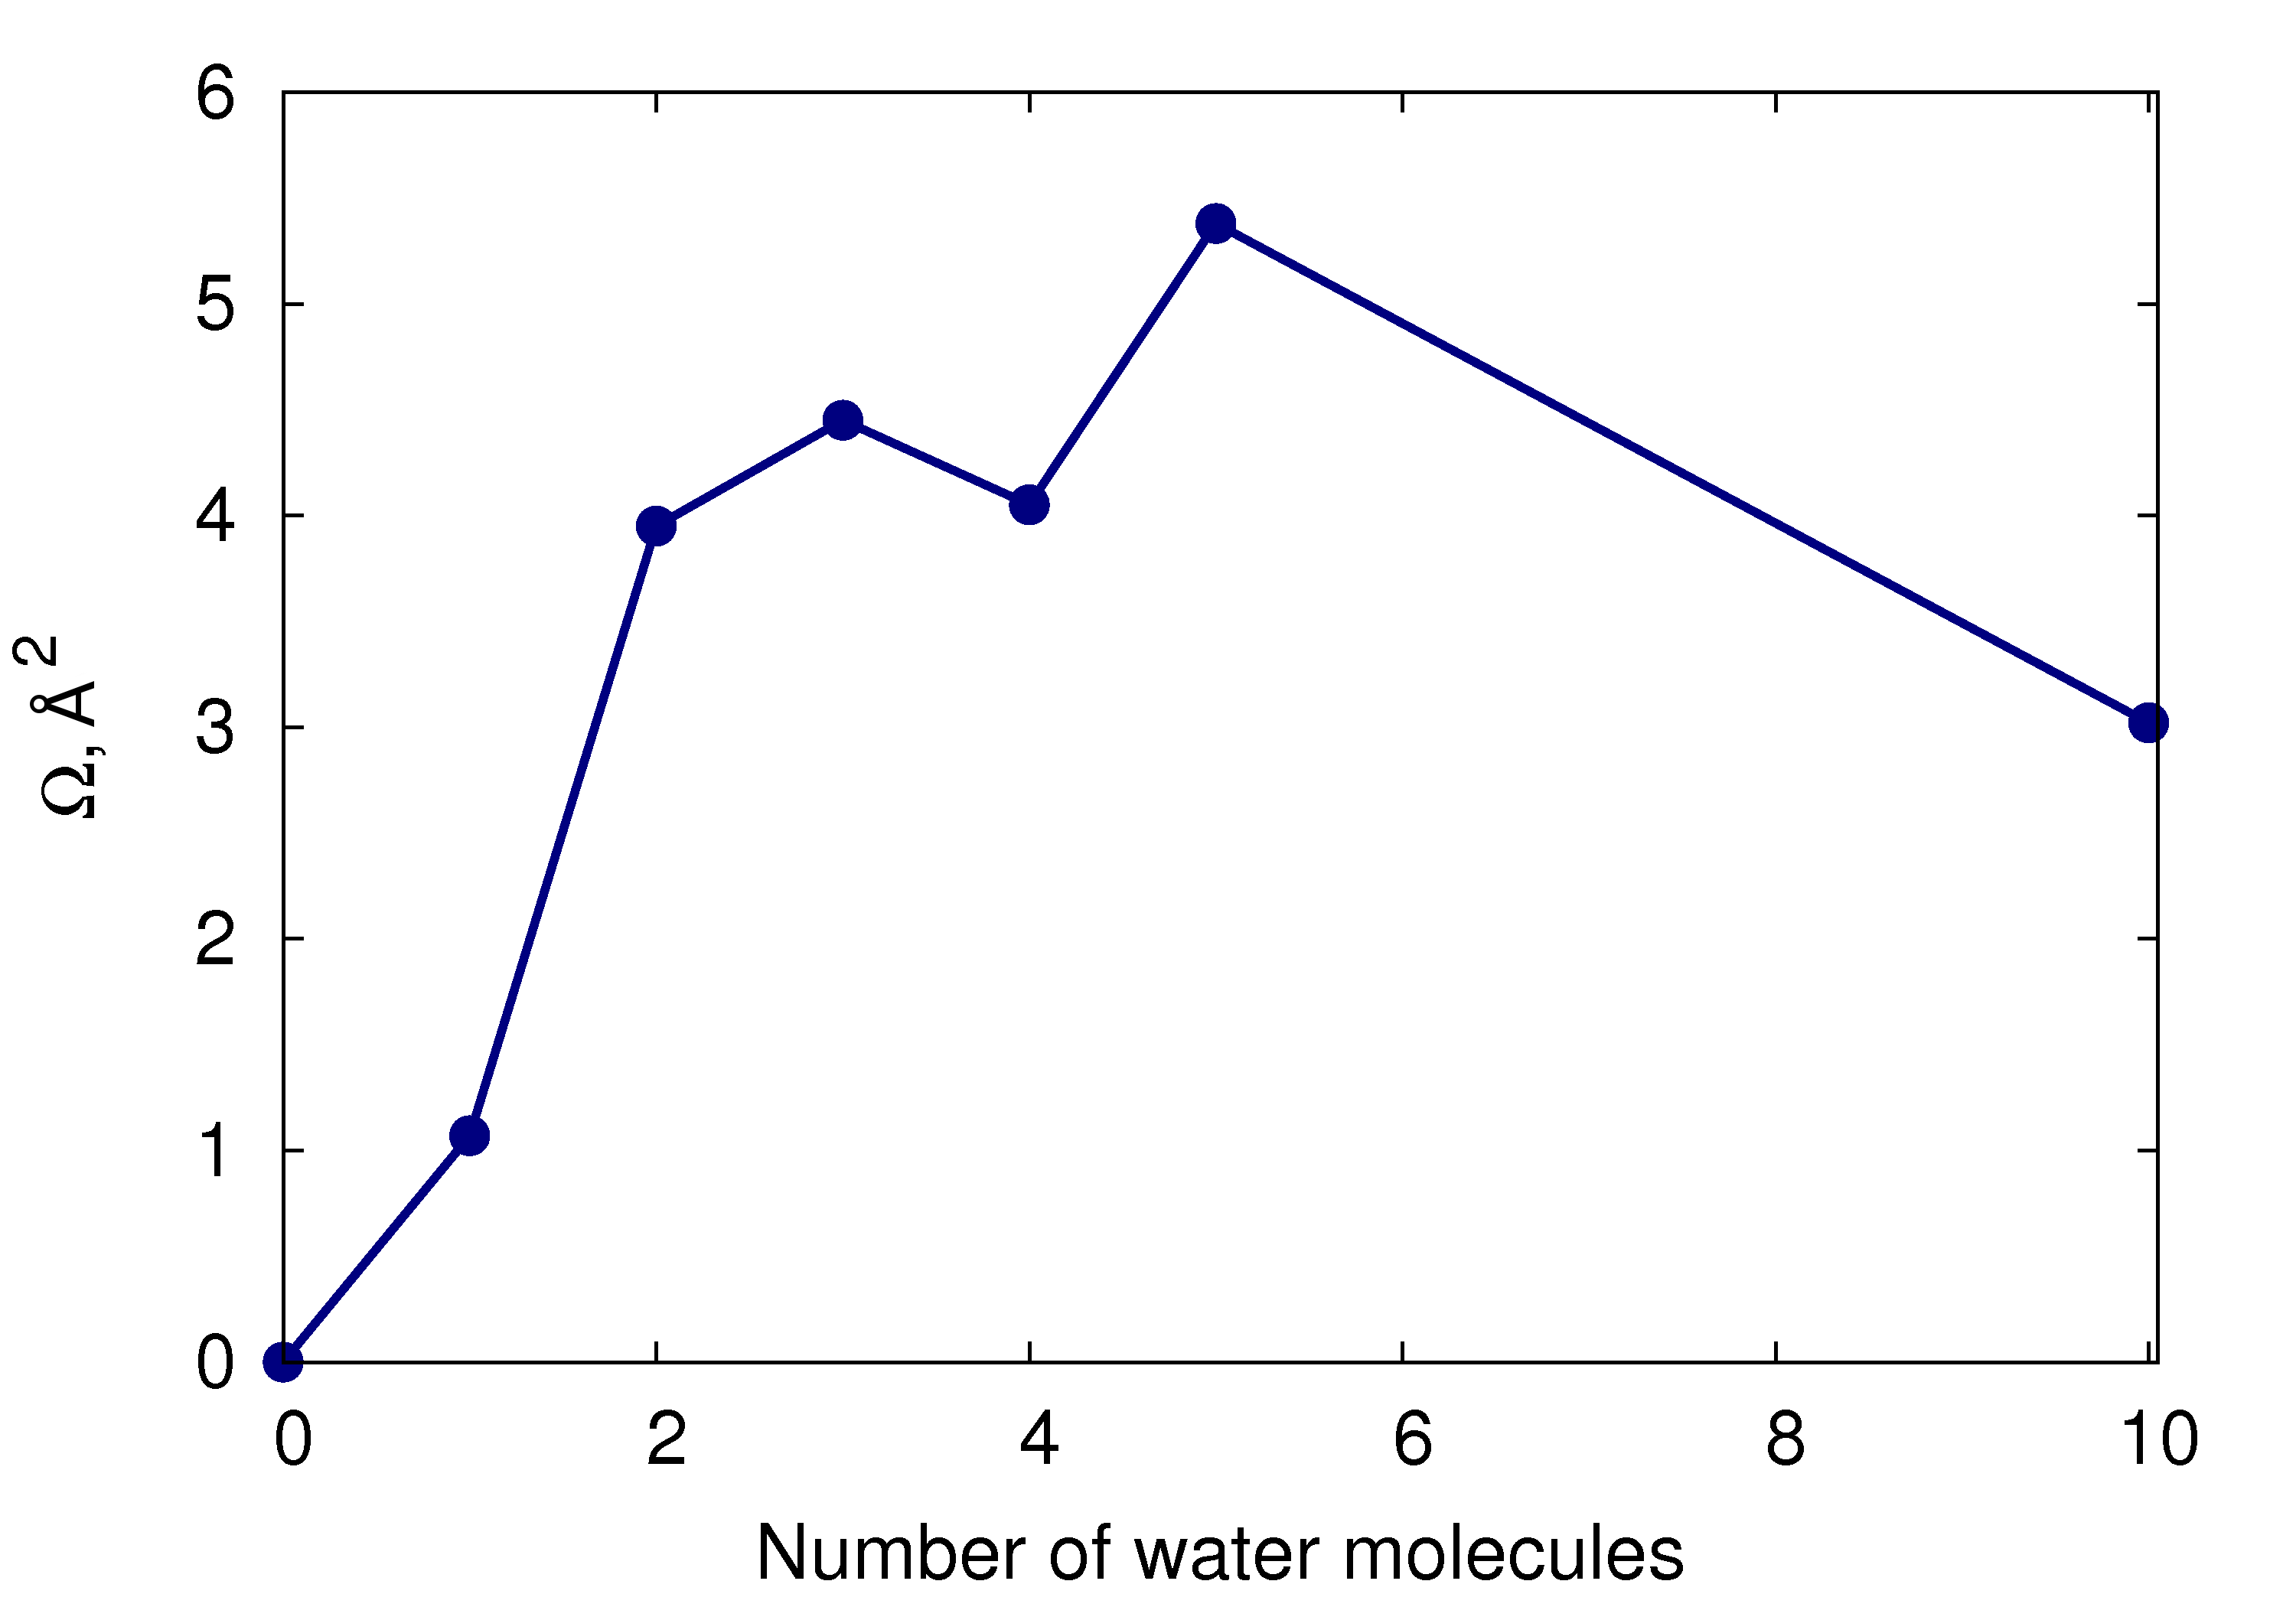
\includegraphics[width=9cm]{HCO_recomb.png}
\end{center}
\caption{Reaction cross section for H + CO formation as a function of water cluster size.
Reprinted with permission from \cite{Korchagina2017a}. Copyright (2017) American Chemical Society.}
\label{recomb}
\end{figure}

\subsection{Adsorption on a PAH surface} \label{PAHice} 

Water clusters in interaction with polycyclic aromatic hydrocarbons (PAHs) are systems of astrophysical and atmospherical interest \cite{Guennoun2011,Guennoun2011bis,Noble2017} that we have been studying in synergy with experimental studies\cite{WaterCorMat_PCCP17}. We first focused on isolated clusters, and then we investigated the influence of the rare gas matrix on their properties, in order to reproduce experimental conditions. This section and next one describe the relevant results that were obtained in this context.


%	- strucural properties
	%- IR Pure MD $\rightarrow$ IR spectra, but positions not accurate for water molecules and thus water clusters. Influence of the environment on the positions could be studied : relative positions are fine if the water - other moleucles intermolecular interactions are well described. Give exmpale of isolated pah-water.    \\

%	- thermodynamical properties : heat capacities of water cluster adsorbed on PAHs \cite{Oliveira2015}
	 % \textcolor{blue}{to be developed ?: PAHs in astrochemistry, interest of the study of their interaction with water clusters }. 
	 (H$_2$O)$_n$-PAH clusters (n=1-10)  are described at the SCC-DFTB level of theory using CM3 charges and dispersion corrections as described in section 1. We determined their structures and interaction energies  at 0\,K \cite{SimonPCCP2012,SimonCOMP2013,SimonJCP2013}, and we studied the influence of the interaction with the PAH surface  on their conformational evolution as a function of temperature \cite{SimonCOMP2013,SimonJCP2013}. This was quantified by the computation of heat capacities through MDPT simulations \cite{Oliveira2015}. The influence of the adsorption on the IR spectra of the PAHs was also investigated. In this section, we present the main results obtained regarding these different aspects.
	 
The computational approach was first benchmarked for  (H$_2$O)$_{1,2}$-C$_6$H$_6$ and   (H$_2$O)$_{1,2}$-C$_{24}$H$_{12}$\cite{SimonPCCP2012}.  For the cluster with one water molecule, the most stable situation corresponds to water molecule interacting through its hydrogen with the $\pi$ ring of the PAH, with a tiny preference for the outer ring in the case of coronene (C$_{24}$H$_{12}$). For the cluster with the water dimer, the most stable situation correspond  to the water dimer interacting on the edge of the PAH with  both $\pi$ and $\sigma$  -interactions. The $\pi$-interaction involves  the H atom of one monomer and the $\pi$ cloud of the PAH whereas the so-called $\sigma$ - interaction is made through the O atom of the other monomer interacting with a H atom of the PAH. 
At 0\,K, we found that the water clusters interacting with PAH maintain their lowest energy structures, dimeric structure for (H$_2$O)$_{2}$ \cite{SimonPCCP2012}, cyclic structures for (H$_2$O)$_n$ (n=3-5)  \cite{SimonJCP2013},  "Prism" isomer in the case of (H$_2$O)$_6$, "Cube" isomer in the case of the (H$_2$O)$_8$ \cite{Oliveira2015}. Studying in quite details the isomeric forms of (H$_2$O)$_6$ adsorbed on coronene, we showed that the adsorption on the surface led to an increase of the density of structures, and that flatter 2 Dimensional structures were favored (see Figure \ref{fig:geoms_w6cor}). This can be accounted for by the occurence of stabilizing $\pi$ interactions between the water monomers and the PAH.
In our first MD/SCC-DFTB studies in the (NVE) ensemble, we noticed that,when increasing the internal energy of the system, we first observe diffusion of the cluster on the PAH surface, then isomerisation into conformers, which were well identified in the case of (H$_2$O)$_6$ \cite{SimonJCP2013}, and finally melting of  (H$_2$O)$_n$, that can be described by a jump of the Lindeman criterion as shown for (H$_2$O)$_8$  \cite{SimonCOMP2013}. When comparing the "kinetic" temperature of the phase change, it was found to be lower for (H$_2$O)$_8$ when the water cluster is adsorbed on the PAH than when it is isolated.
	
	
\begin{figure}[!ht]
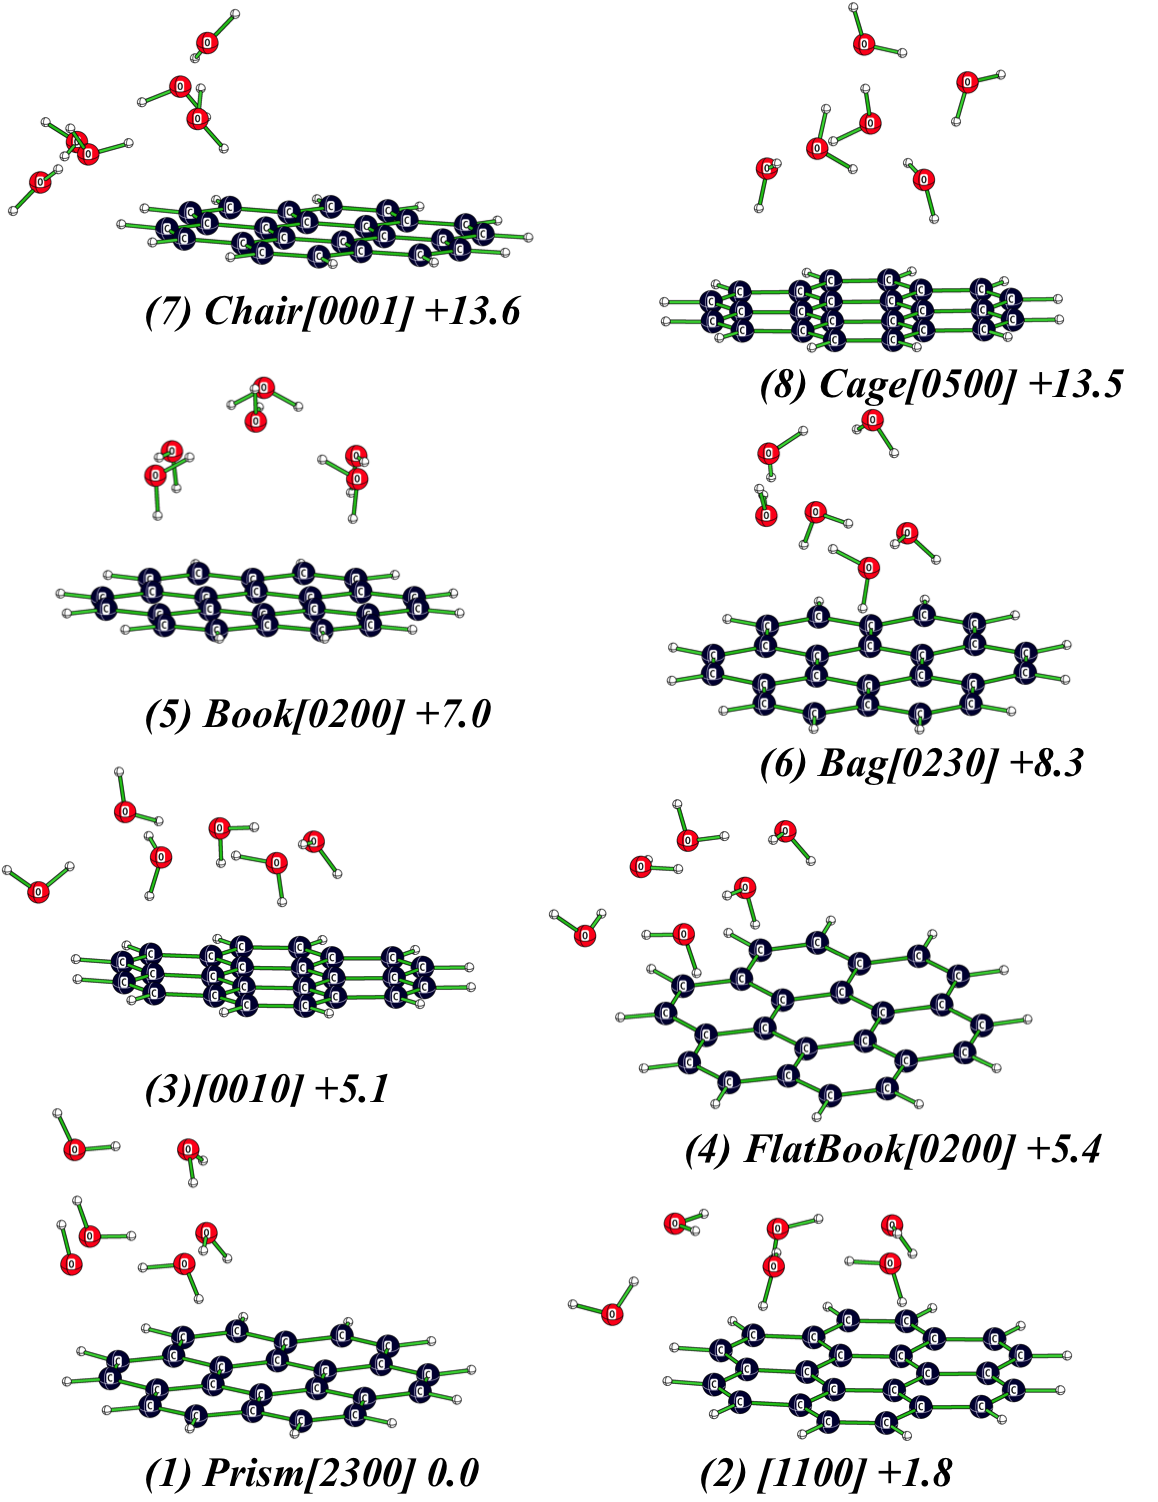
\includegraphics[width=12cm]{geoms_w6cor.png}
\caption{Optimized geometries of the isomers of (H$_2$O)$_6$C$_{24}$H$_{12}$ determined at the SCC-DFTB level using CM3 charges and dispersion corrections. The relative energies (in kJ.mol$^{-1}$) with respect to the most stable isomer are also reported. The [mnop] nomenclature is similar to that of Figure\ref{fig:geoms_w6} }
\label{fig:geoms_w6cor}
\end{figure}

	
	
	These first MD/SCC-DFTB studies were quantified by the determination of heat capacities for (H$_2$O)$_{6,8}$ adsorbed on coronene and circumcoronene (see Figure~\ref{fig:capa_WnPAH}). The results were complemented with the population evolution of the different isomers as a function of temperature \cite{Oliveira2015}. We showed that the phase change temperature decreases for (H$_2$O)$_8$ when it is adsorbed on a PAH surface whereas in the case of (H$_2$O)$_6$, the results are dependent on the PAH.  This is interpreted in terms of density of isomers as a function of temperature : similarly to the isolated water clusters' case, although the lowest energy structure of (H$_2$O)$_8$ is a cube with a few other isomers appearing at 120-150K  in the case of adsorption on circumcoronene (Fig. 10 in ref. \cite{Oliveira2015}), a larger variety of low energy isomers are formed in the case of (H$_2$O)$_6$, starting at 90 K (Fig. 8 in ref.  \cite{Oliveira2015}).
	
	%	Study of water-PAH isolated complexes, isolated \cite{Oliveira2015,SimonCOMP2013,SimonJCP2013}. 
	%	Use of CM3 charges : benchmark. \\
		%Influence of the adsorption of the PAH on the structures of water clusters as a fonction of temperature : conformation evolution : qualitative and  quantitative (heat capacities). \\
		
		 \begin{figure}[!ht]
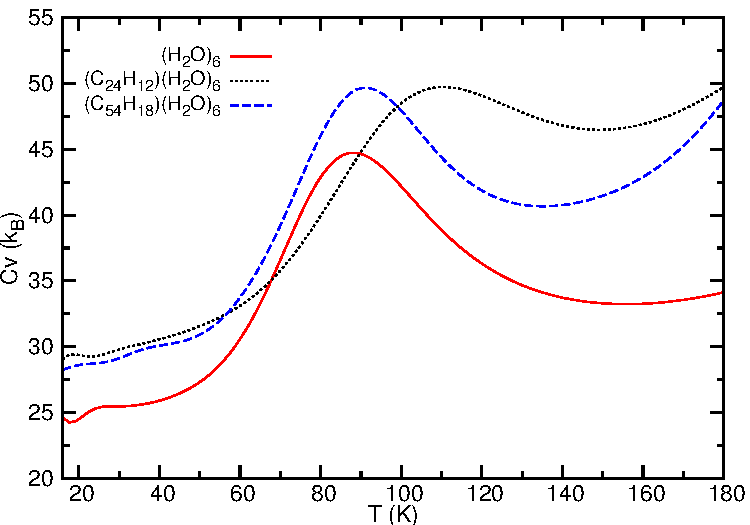
\includegraphics[width=7cm]{CapaW6PAH.pdf}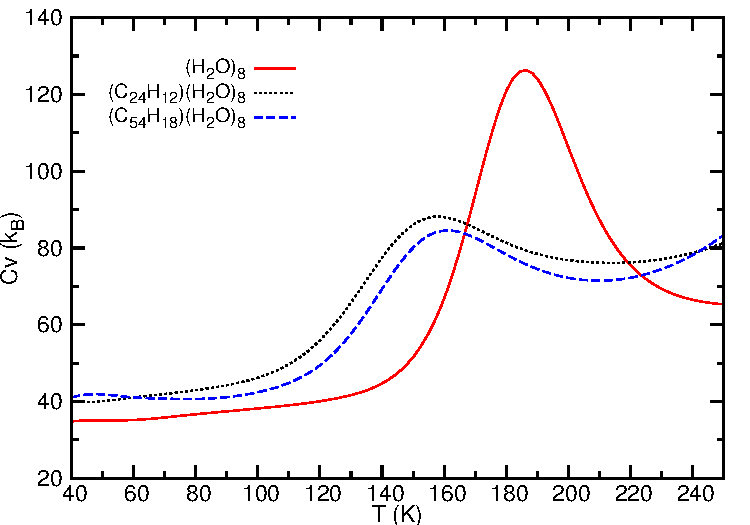
\includegraphics[width=7cm]{CapaW8PAH.pdf}
\caption{Heat capacity curves, obtained form PTMD/SCC-DFTB simulations, for two water clusters, (H$_2$O)$_{6}$ (left) and  (H$_2$O)$_{8}$ (right), isolated and adsorbed on two compact PAHs, namely coronene $C_{ 24}H_{12}$ and circumcoronene $C_{ 54}H_{18}$.  Reprinted with permission of the Royal Society of Chemistry from ref. \cite{Oliveira2015}.}
\label{fig:capa_WnPAH}
\end{figure}	
		
		
		From the study of the evolution of the anharmonic IR spectra of $(C_{ 24}H_{12})(H_{2}O)_{n}$ (n=1-3,6,8) as a function of internal energy  %was investigated, 
		qualitative and quantitative information could be retrieved. Globally, redshifts, broadenings and merging of bands were observed. Anharmonicity factors could be determined for (n=1,2).  
		For instance, the anharmonicity of the $\nu_{1}$ symmetric stretching mode of $H_{2}O$ was found to decrease when adsorbed on $C_{ 24}H_{12}$, whereas the anharmonicity of the $\nu_{2}$ bending  mode was found to be hardly affected. However, the complexity of the spectrum of $(C_{ 24}H_{12})(H_{2}O)_{n}$ for n$>$1  prevents a reliable quantitative study of the water modes. Nevertheless, the increased anharmonicity of the C-H out-of-plane bending mode ($\gamma_{CH}$ mode) of $C_{ 24}H_{12}$ when $(H_{2}O)_{2}$, or $(H_{2}O)_{3}$ in its linear conformation, or even  $(H_{2}O)_{6}$ under its prismatic (lowest energy) form,  is adsorbed, could be used as a  signature for the edge-coordination of the water clusters on the coronene molecule. This is an illustration that, although obviously errors (sometimes significant) can be found on the absolute positions of the IR modes, their evolution as a function of internal energy should be useful to fingerprint conformational changes.
		
		We also showed that, at low temperatures, the IR spectra of isolated and adsorbed water clusters for (n=3,6) could be distinguished. However, as the temperature increases, the differences are quenched. In the temperature evolution of the IR spectra of $(C_{24}H_{12})(H_{2}O)_{3,6}$ complexes, we observe the merge of the water cluster bands, which illustrates the isomerisation processes.  The sudy of  the influence of the adsorption of $(H_{2}O)_{8}$  on coronene on the IR spectrum at low (kinetic) temperature revealed that the IR spectrum gets more complex as: (i) degeneracy is quenched leading to band splittings ; (ii) new modes are activated ; and (iii) some modes of the water cluster couple to the modes of coronene. The analysis of anharmonic IR spectra shows that, for all the studied internal energies (prior to the evaporation of the cluster), the spectra of bare and adsorbed $(H_{2}O)_{8}$ can be distinguished. It is also interesting to quote that, at any (kinetic) temperature, even when the "melting" threshold  is reached, the spectrum of $(C_{24}H_{12})_{0,1}(H_{2}O)_{8}$ is clearly different from that of $(C_{24}H_{12})_{0,1}(H_{2}O)_{6}$, and thus a signature of the structure of the (finite)-size cluster.

		
		
	%	We also studied water clusters in an environment constituted of a rare gas matrix, in synergy with experimental studies.  \\

\subsection{ Embedding in a cryogenic matrix }
As mentionned in section 1, a hybrid DFTB/FF scheme was developed to describe the interaction between hydrocarbons and water with rare-gas atoms \cite{Iftner_JCP2014,WaterMat_JPCA2015}. Using this scheme, we studied the influence of an argon matrix on the structures, stabilities and IR spectra of: (i)  water molecules and clusters \cite{WaterMat_JPCA2015} ; and (ii) $(C_{6}H_{6})(H_{2}O)_{1,2}$ and   $(C_{24}H_{12})(H_{2}O)_{1,2}$   \cite{WaterCorMat_PCCP17}.

In our approach, $(H_{2}O)_{n}$  and PAH-$(H_{2}O)_{n}$ are described with SCC-DFTB, using CM3 charges and dispersion corrections. The argon matrix is represented by a large cluster ($\sim$ 350 to 1050 Ar atoms) organized in a face centered cubic (fcc) crystalline structure, in which the impurity (namely $(H_{2}O)_{n}$  or  PAH-$(H_{2}O)_{n}$) is inserted after removing the minimum number of Ar atoms, ie after the creation of a minimal size vacancy.
% This relaxed matrix geometry - including the vacancy- is considered as the reference and its energy will be labelled  $E_{mat}^*$. In the following, $E_{(H_2O)_n}$ is the SCC-DFTB energy of the optimized isolated water cluster,
%and $E_{(H_2O)_n/Ar}$  the energy of the total system (water cluster embedded  the matrix) in its SCC-DFTB/FF geometry.

Structures and energetics are determined after local optimization. 
We found that  structures of 2\,D water clusters (n=1-4) are hardly modified by the embedding in the matrix whereas in the case of 3\,D structures (n=6), noticeable distortions may occur. This is particularly observed for  the 6-membered ring isomers (namely Chair and Boat) that become planar, while the two 4-member rings of the Bag structure become planar and orthogonal (one ring in a reticular plane of the $fcc$ lattice).

We defined several quantities to  describe the energetics of PAH$_{0,1}$(H$_2$O)$_n$ clusters embedded in the $Ar$ matrix (see section 3.2 of ref  \cite{WaterMat_JPCA2015}), in particular the substitution energy  $E_{sub}$ of a vacancy by the  PAH$_{0,1}$(H$_2$O)$_n$  cluster, relative to the $n$ independent water molecules, and to the isolated PAH if there is: 

\begin{equation}
E_{sub}=E_{PAH_{0,1}(H_2O)_n/Ar}-E_{mat}^*-nE_{(H_2O)}-E_{PAH_{0,1}}
\end{equation}
where  $E_{(H_2O)_n/Ar}$  is the energy of the total system (water cluster embedded  the matrix) in its SCC-DFTB/FF geometry, $E_{mat}^*$ the FF energy of the relaxed matrix geometry - including the vacancy-, $E_{(H_2O)}$  and $E_{PAH_{0,1}}$ the SCC-DFTB energies of the isolated monomers. Such a quantity allows to compare various vacancies and isomers for a given cluster size  and does not depend on matrix size, provided convergency is reached (sufficiently large finite matrix).

Using this quantity, we determined the stability of (H$_2$O)$_n$ clusters (n=2,6) inside an argon matrix. Regarding the isomers of (H$_2$O)$_6$, we showed the competition between the prism, cage and bag isomers whereas the 6-membered ring isomers we found to be higher in energy.  In the case of PAH-(H$_2$O) clusters, a $\pi$ complex was found to the be most stable for benzene whereas a $\sigma$ complex was found as the most stable isomer in the case of coronene, which is not the case of the gas phase where $\pi$ complexes are more stable for any PAH size. We note that, in our model, the most stable situation (for the PAH isolated or in interaction with water) corresponds to the PAH occupying the [111] crystal plane  with a vacancy of 3 Ar atoms for benzene and a vacancy of 7 Ar atoms in the case of coronene.

	 \begin{figure}[!ht]
	 \begin{center}
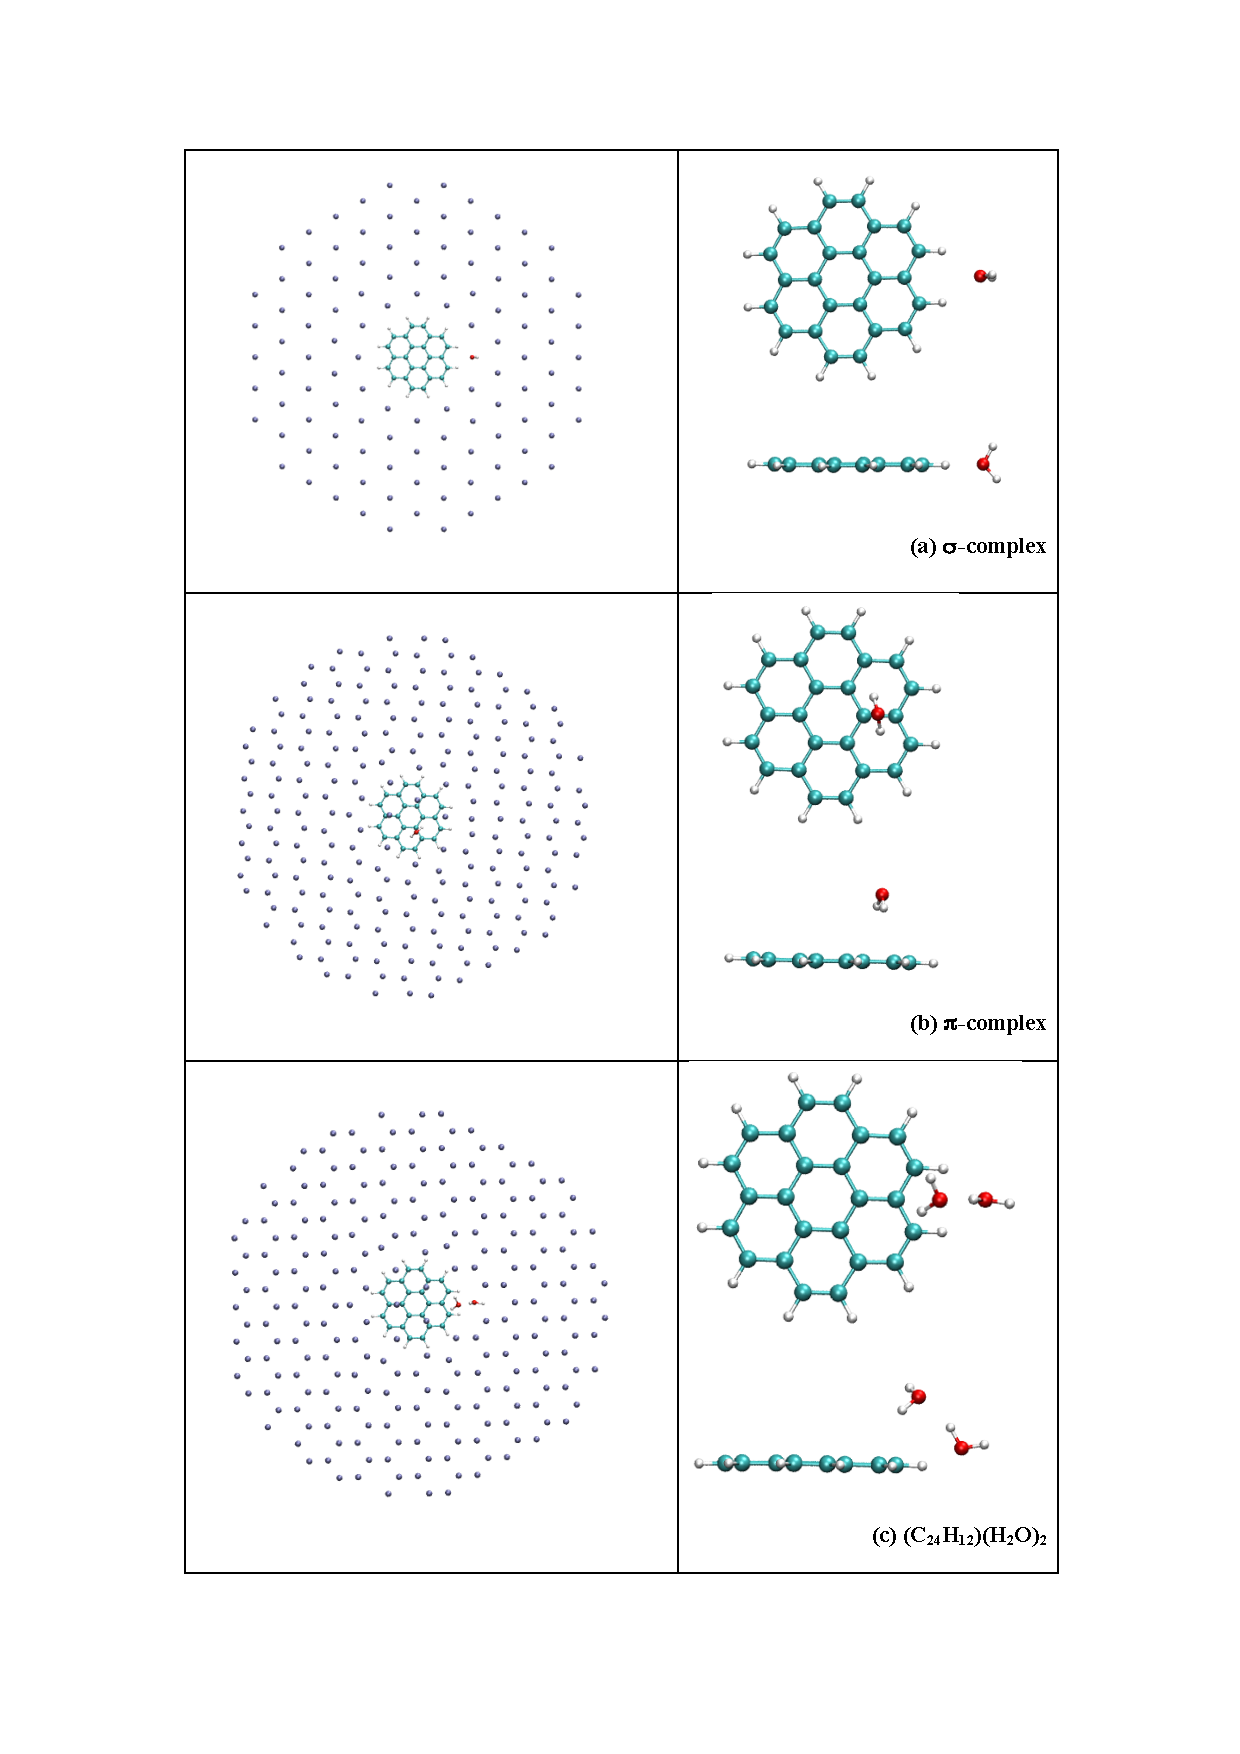
\includegraphics[width=11cm]{geoms_mat.pdf}
 \end{center}
\caption{DFTB/FF optimised geometries of coronene-water complexes in an argon matrix (a) (C$_{24}$H$_{12}$)(H$_2$O) $\sigma$-complex, (b) (C$_{24}$H$_{12}$)(H$_2$O) $\pi$-complex, (c) $(C_{24}H_{12})(H_{2}O)_{2}$ complex. Left column: top views with one (a) or two (b and c) layers of Ar atoms; right column: zoom of the $(C_{24}H_{12})(H_{2}O)_{1,2}$ molecular system in its geometry inside the matrix (top and side views). Reprinted with permission of the Royal Society of Chemistry from ref. \cite{WaterCorMat_PCCP17}  (http://dx.doi.org/10.1039/c6cp08559h)  }
\label{fig:geoms_mat}
\end{figure}

 
 Starting from the most stable locally optimized structures, we achieved MD simulations to obtain IR spectra at $\sim$10\,K. 
 %We found that the water molecule was rotating inside the matrix, and that leads to red shifts and broadedning of the IE spectrum. This is   in line experimental data for low water concentration. Regarding the water dimer, the rotation-torsion is oberved, whereas no global motion is observed for larger clusters, trapped in the matrix lattice.   
 The behavior of the $(H_{2}O)_{n}$/Ar systems at a kinetic temperature of $\sim$10\,K is in line with existing experimental data: the rotation of the water monomer is observed, as well as the rotation-torsion structure of the dimer, whereas no global motion of the larger clusters is found  to occur.  The IR spectra of $(H_2O)_n$/$Ar$ systems present broader and more structured bands than those of bare $(H_2O)_n$ clusters.  Some new bands also appear due to the different environment seen by the H atoms of the water molecules during their internal rotation motions. For all clusters, the position of the $\nu_2$ band is hardly modified whereas the $\nu_1$ and $\nu_3$ (asymetric stretching mode) bands are redshifted. In the case of the water monomer and dimers, the shift  values are in fair agreement with the experimental data. 
The case of the water hexamer is the most complex as many isomers are likely to coexist. The comparison of the computed spectra with the experimental spectra by Ceponkus and co-workers  \cite{Ceponkus2012}. %\cite{Ceponkus2012}
 tends to confirm the presence of the Cage (and probably the Cycle) isomer, but given the approximations within our scheme, no  unambiguous assignment can be achieved.
 
Regarding the IR spectra of the $(C_{24}H_{12})(H_{2}O)_{1,2}$ , the $\sigma$ coordination, which appears to be favored energetically,  leads to a larger blue shift for the $\gamma_{CH}$  mode of the PAH than  $\pi$ coordination and this shift appears to increase with cluster size. This is in line with experimental results \cite{WaterCorMat_PCCP17}. An important point is that such a $\sigma$ interaction is expected to favor photochemical reactions between water and coronene at the edge of the coronene molecule \cite{Noble2017}.
   
  \begin{figure}[!ht]
   \begin{center}
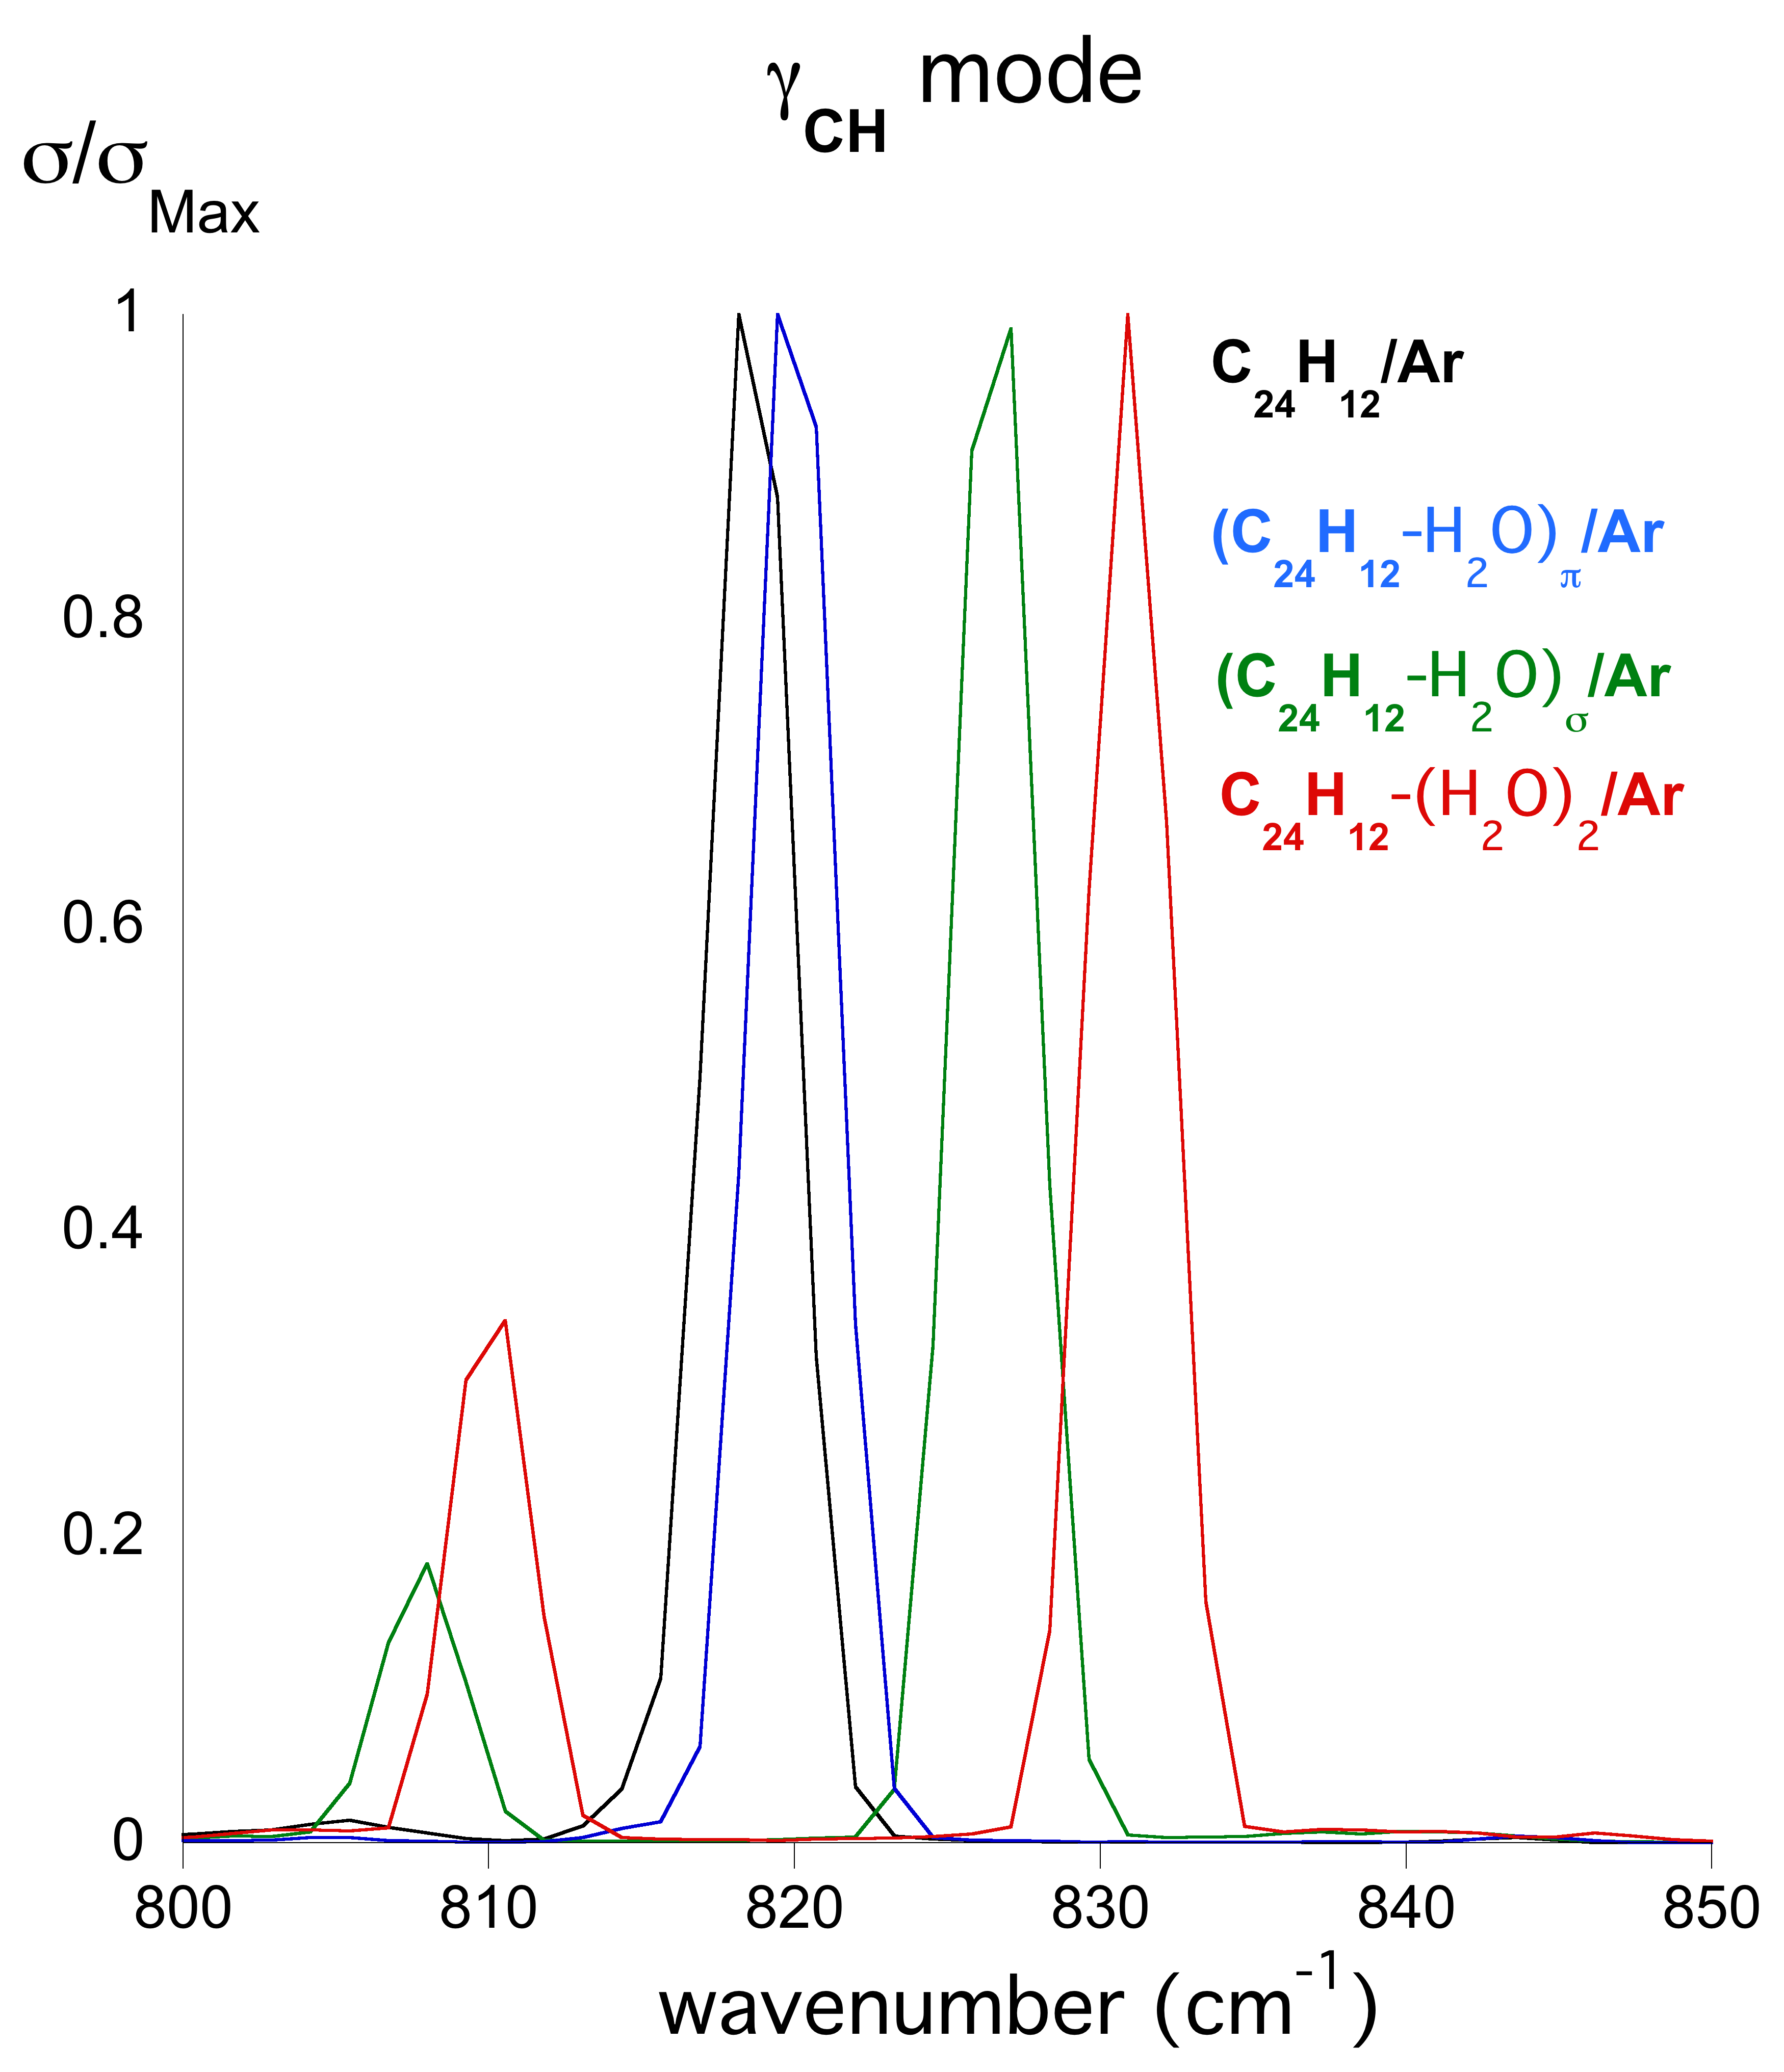
\includegraphics[width=9cm]{comp_gCH.png}
\end{center}
\caption{Dynamic spectra of coronene-water complexes at 10\,K , obtained form MD/SCC-DFTB simulations : zoom on the $\gamma_{CH}$  mode. Adapted with permission of the Royal Society of Chemistry from ref. \cite{WaterCorMat_PCCP17}  (http://dx.doi.org/10.1039/c6cp08559h) }
\label{fig:irmat}
\end{figure}

\subsection{Toward infinite water systems } \label{infinite}

\subsubsection{Description of PAHs adsorbed on water ice } 

In dense and cold  molecular clouds of interstellar space, PAHs are likely to condense onto water ice \cite{Bowman2011}. These systems may be submitted to UV irradiation or energetic particle bombardment, likely to lead to a rich heterogenous chemistry occurring at the surface of the water ice \cite{chemRev2016}. This motivated experimental studies \cite{barros17,Bernstein2001,Bernstein2007,Bernstein1999,Bouwman2009,Bowman2010,Guennoun2011,Guennoun2011bis} and it was proposed that the photo-initiated reaction of PAHs with water on the ice surface, even at low energy, could be ion-mediated \cite{Bouwman2009}. Besides, experimental investigations combined with theoretical studies have shown that  the interaction with the ice led to a decrease of the ionisation energy of the PAH by  1.5 to  2\,eV \cite{Gudipati2004,Woon_2004}, the resulting PAH cations being stable over time  \cite{Gudipati2006}. Theoretical studies dealing with the ionisation of PAH on the ice surface are scarce - we can cite one performed with the Polarized Continuum model (PCM) \cite{Woon_2004}- , due to the need to treat both a large system and the explicit electronic structure in order to describe the PAH-ice systems in their neutral and charged states. Furthermore, one has to counter the self interaction issue within all DFT-base approaches.

This motivated us to study the effect of ice on the ionization energies of PAH using the SCC-DFTB and C-DFTB scheme with modified Mulliken charges WMull and dispersion corrections. 
In order to do so, we used MD/FF low energy structures  \cite{Michoulier18a} are starting point geometries to build a finite-size  PAH-water ice system further locally optimized at the SCC-DFTB level. In our model  water ice is represented by a cluster of about 150 water molecules with the 100 more external molecules frozen during the optimization process (to main the density). We studied a series of PAH from naphthalene (C$_{10}$H$_{8}$) to ovalene (C$_{32}$H$_{14}$) on different types of ices, crystalline (hexagonal Ih and cubic Ic) and amorphous (low density amorphous LDA). More information can be found in ref. \cite{Michoulier18b}. 
We showed in particular the dependence of the IP with local structure  (see Figs.~\ref{fig:IP} and ~\ref{fig:config}). The presence of OH dangling bonds at the surface of water ice interacting with the PAH tends to favor an increase of the IP whereas the interactions between oxygen atoms at the water ice surface and the PAH tends to decrease it. This was quantified  by establishing correlation laws between atomic pair interaction energies and the IP variation  (see Fig. 7 in ref. \cite{Michoulier18b}.).


%increases/decreases  with respect to that of the isolated PAH in the presence/absence of dangling O-H at the surface interacting with the PAH (see Fig.~\ref{fig:config}). 

  \begin{figure}[!ht]
   \begin{center}
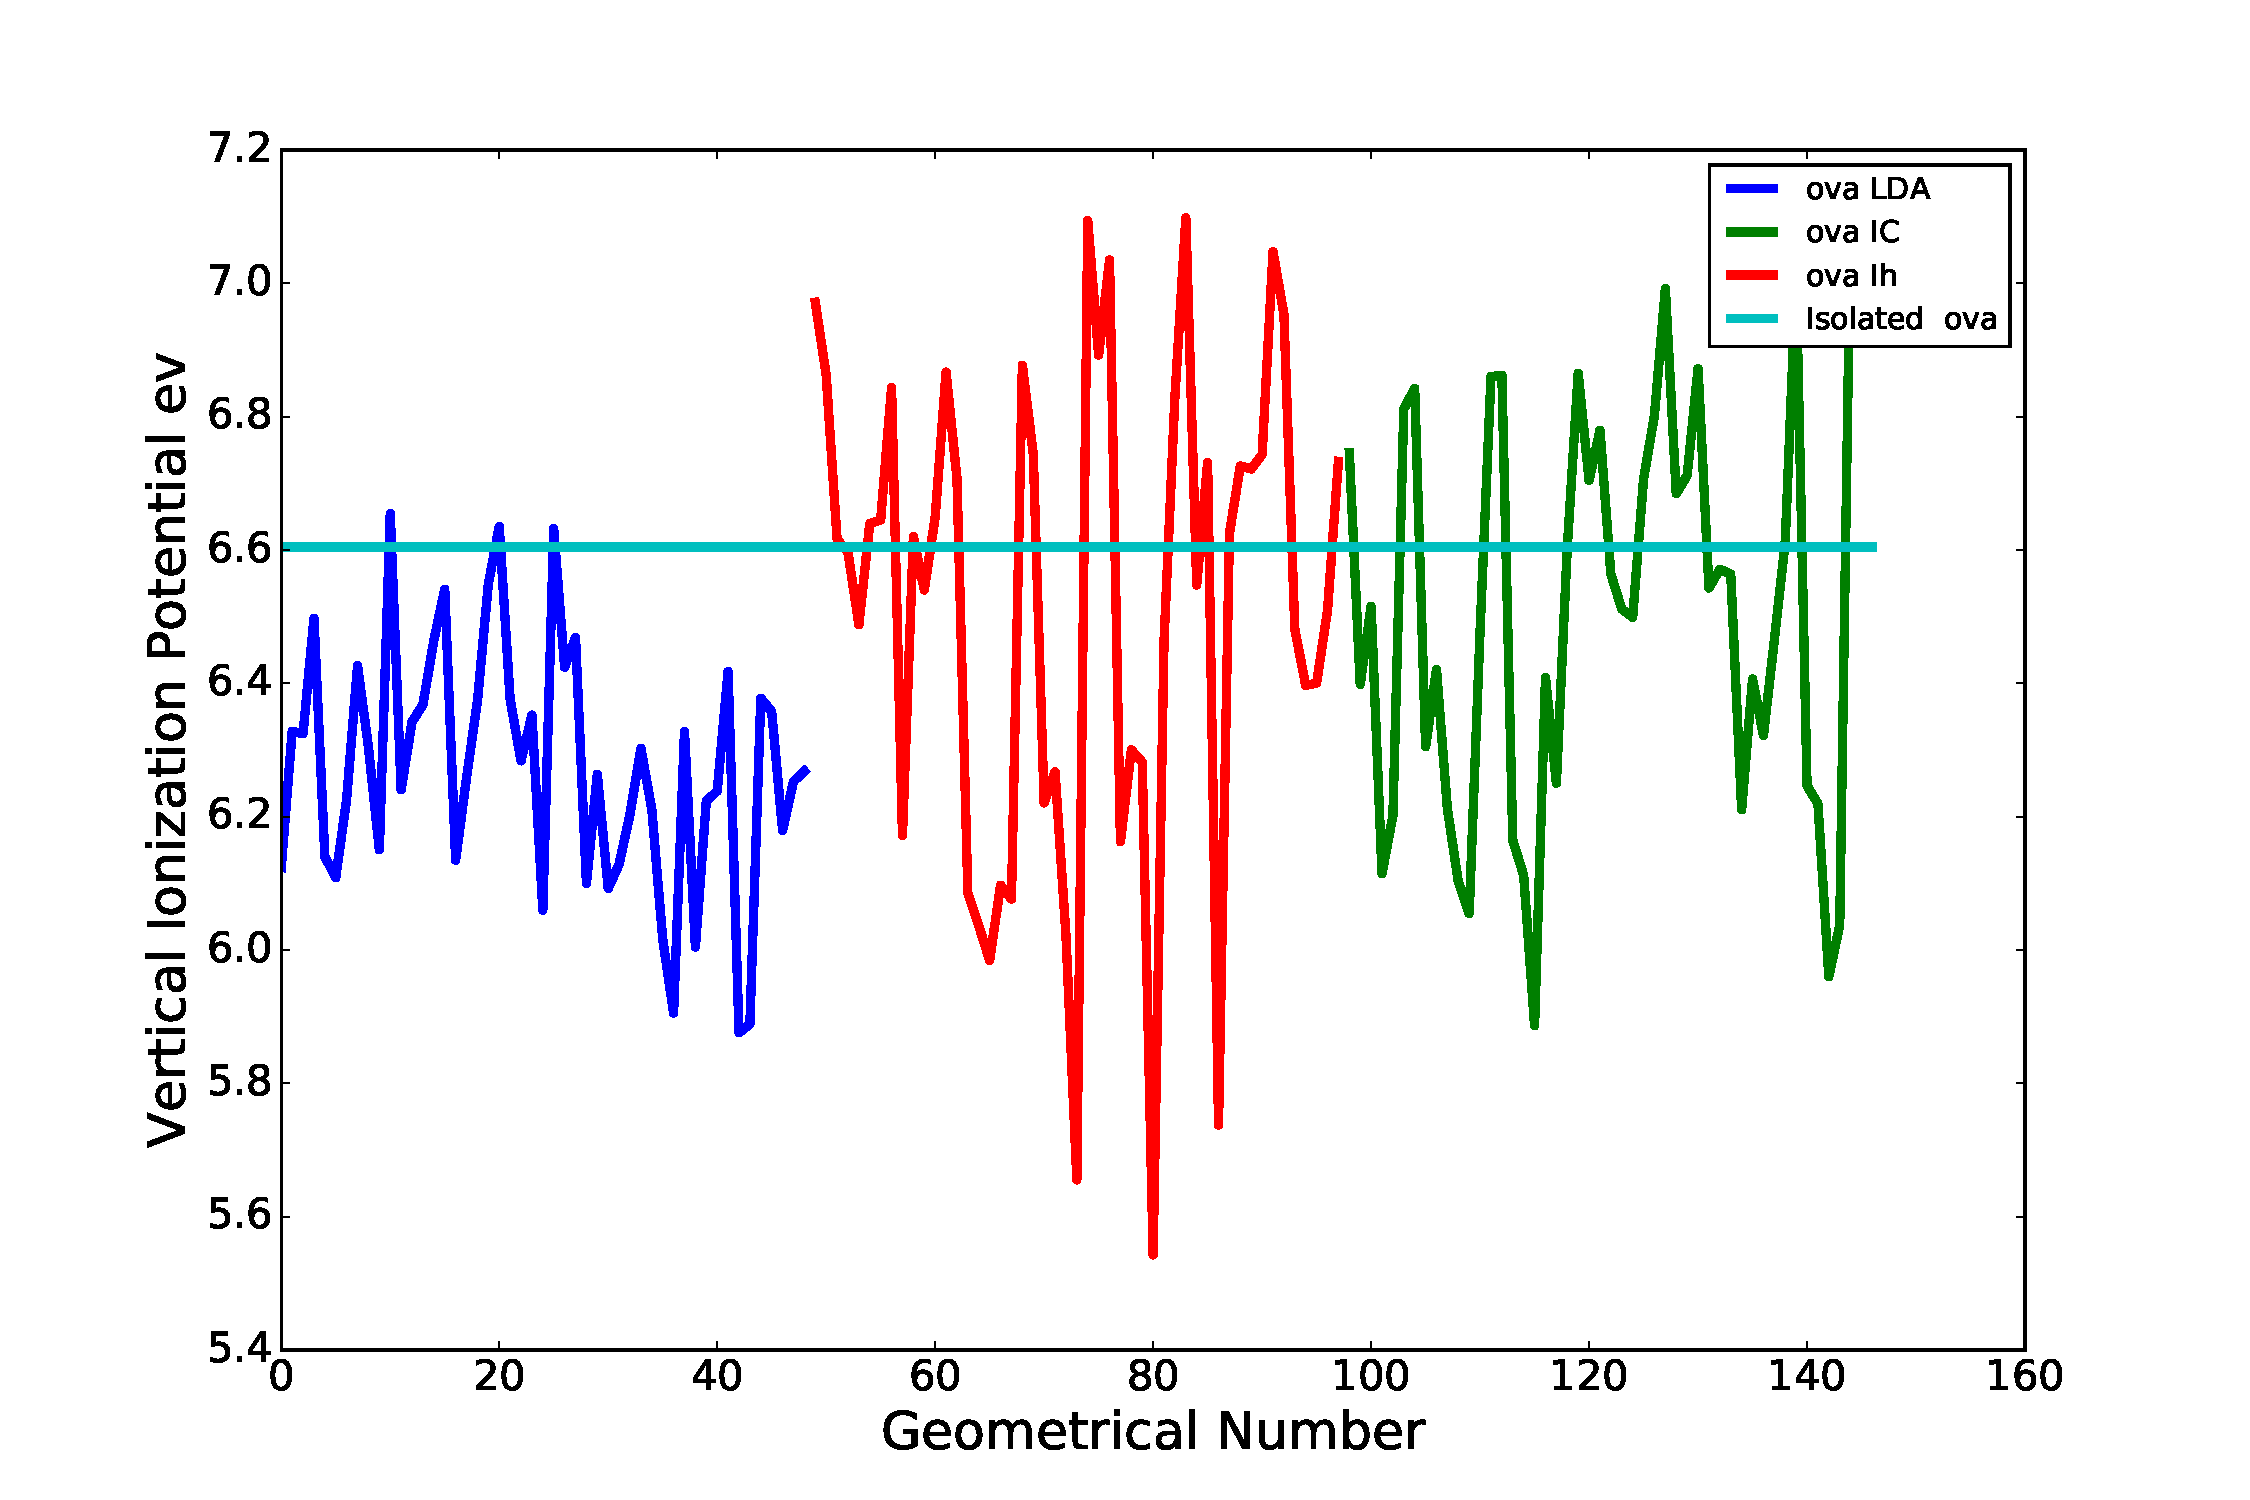
\includegraphics[width=14cm]{ova_LDA_IC_IH.pdf}
\end{center}
\caption{Evolution of the IP of ovalene adsorbed on water ice for three types of ice (LDA, Ih and Ic) as a function of the structural configuration (49 for each ovalene-water ice duet, see reference \cite{Michoulier18b} for more information )}
\label{fig:IP}
\end{figure}


\begin{figure}[!ht]
   \begin{center}
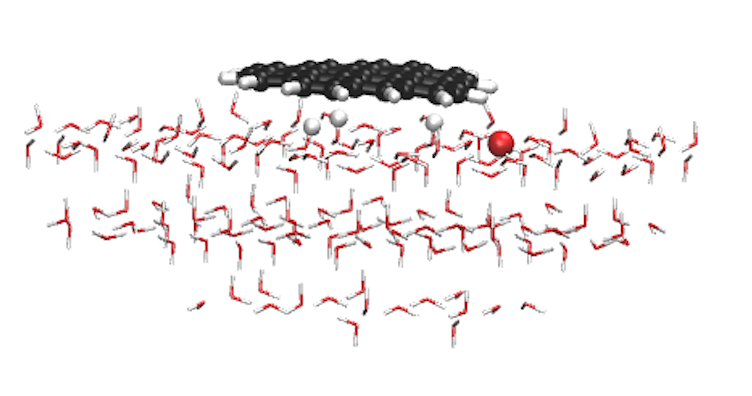
\includegraphics[width=9cm]{ova_Ih_31_min.png} 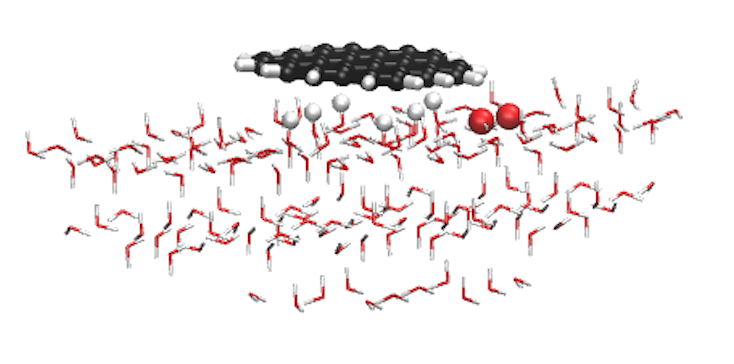
\includegraphics[width=9cm]{ova_Ih_34_max.png}
\end{center}
\caption{Geometrical configurations of ovalene on hexagonal ice leading to the minimum (top) and maximum (bottom) ionization potential. The dangling hydrogens and the oxygen atoms on the surface of ice, interacting with the PAH, are highlighted. }
\label{fig:config}
\end{figure}

Our conclusion is that the small magnitude of the IP variation, that is at most 0.8 eV for amorphous ice (the experimental type of ice) cannot account for the experimental results. In fact, the electron ejected for the PAH could be transfered to the water ice or to recombine with impurities such as the OH radicals. Substracting the electron affinity of ice (1.65-3.5 eV\cite{Novakov2004}) or that of OH radicals trapped in water ice (5.06\,eV \cite{Woon_2004})  to the computed IP lowering could account for experimental results. However, our SCC-DFTB approach in its current form does not allow us to study PAH$^{+}$-H$_2$O$^{-}$ system, H$_2$O$^{-}$ being not properly described.  Another hypothesis is that the electron could be transfered onto the ice through the population of electronic excited states \cite{Noble2017}, and we are currently testing this hypothesis by means of multireference wavefunction calculations. Another current study concerns the influence of the adsorption of the PAH on the vibration of the dangling OH bonds, which is a topic of astrophysical relevance.

\subsubsection{Description of liquid water}

Finally, a number of studies have been devoted to the development and validation of a SCC-DFTB parametrization to
describe liquid water \cite{Maupin2010,Goyal2011,Choi2013,Liang2014,Goyal2014}. This represents an exciting research topic as the
possibility to properly describe this system at a rather low computational cost would allow for a variety of subsequent
studies. However, this is not straightforward as modelling liquid water presents a number of challenges even
at the DFT level \cite{Sprik1996, SilvestrellliLuigiParrinello1999,GrossmanSchweglerDraegerGygiGalli2003,Chen2003,Ramirez2004,
KuoMundyMcGrathSiepmannVandeVondeleSprikHutterKleinMohamedKrackParrinello2004, LeeTuckerman2006b,
Zhang2010,Laage2011,Heyden2012,Kuhne2013,Hassanali2014,Gillan2016,Gasparotto2016,Miceli:2016hy,Chen:2017jn}. In particular, it is well known that simulations based on the generalized-gradient approximation, for instance using the PBE functional, lead to an
over-structured liquid water \cite{Sit2005}. It is not the scope of the present article to review the whole literature focusing on
liquid water, however, it has appeared since a decade that a correct description at the DFT level would involve a
subtle balance between quality of the exchange-correlation functional \cite{VandeVondeleMohamedKrackHutterSprikParrinello2005,Todora2006,GuidonSchiffmanHutterVandeVondele2008,Zhang2011,DiStasio2014,Ambrosio:2016er,Pestana:2017fy}, description of dispersion interactions \cite{LinSeitsonenCoutinhoMauricioTavernelliRothlisberger2009,AndreasKelkkanenAndreWikfeldtJakobJorgenLArsJacobsenNillssonJens2011,Zhang2011A,JohnchiereSeitsonenFerlatSaittaVuilleumier2011} and inclusion of nuclear quantum effects \cite{MorroneCar2008,Ceriotti2013,Fritsch2014,Ceriotti2016}. 
For instance, DiStasio \textit{et al.} conducted an important study where the  first two parameters were carefully taken into account.
It led to theoretical pair radial distribution functions in very good agreement with experimental data \cite{DiStasio2014}.

The approximations of the SCC-DFTB formalism add an additional complexity to the description of liquid water. Indeed, the
first SCC-DFTB study was proposed by Maupin \textit{et al.} using the original formulation of SCC-DFTB as well as a modified
formulation that includes a hydrogen bonding damping function \cite{Maupin2010}. On the one hand, the structure of the liquid in the
second and third solvation shells are very poorly described as revealed by flat oxygen-oxygen radial distribution functions
obtained using the two approaches. On the other hand, the first solvation shell is overstructured. This leads to a self-diffusion
coefficient of water much too high as compared to the experiment. Further studies were conducted to improve those
deficiencies in both the SCC-DFTB or DFTB3 formalisms \cite{Goyal2011,Goyal2014} although no fully satisfactory 
result has been obtained so far \cite{Choi2013,Liang2014}. In order to go a step further in the development of a 
SCC-DFTB potential accurate enough to describe liquid water, we have implemented the Weighted Mulliken charges 
presented in section~\ref{method} in the periodic part of the deMonNano code to rationalise the influence of 
optimized charges on the description of liquid water. Figure~\ref{liquidwater} presents the oxygen-oxygen pair radial
distribution function ($g(r)$) obtained  with the original Mulliken charges and the WMull charges with t$_{OH}$ = 0.39,
\textit{i.e.} the same value used by Michoulier \textit{et al.} to study bare water clusters in section~\ref{bare_water}
\cite{Michoulier18b}. In both cases, the curve was obtained from a classical trajectory that consisted in 128 water molecules in a
15.64~\AA~cubic box. Simulations were performed in the canonical ensemble at 300~K using a global Nose-Hoover chain of five
thermostats with frequencies of 800 cm$^{-1}$ \cite{Nose1984,Hoover1985}. Both simulations were equilibrated during
20~ps at 300~K before 100~ps of production run and were performed using a 0.5~fs time step. As can be seen in
Figure~\ref{liquidwater}, the WMull charges greatly improve the liquid structure in the second and third solvation shells. Indeed,
above 3~\AA, the theoretical curve is very close to the experimental one. However, the increase of t$_{OH}$ also leads
to an increase of the maximum of the first peak centered at 2.75~\AA. So, although an optimized definition of the atomic
charges does not provide a perfect description of liquid water structure, it greatly improves it with respect to the original
Mulliken scheme.  

\begin{figure}
\begin{center}
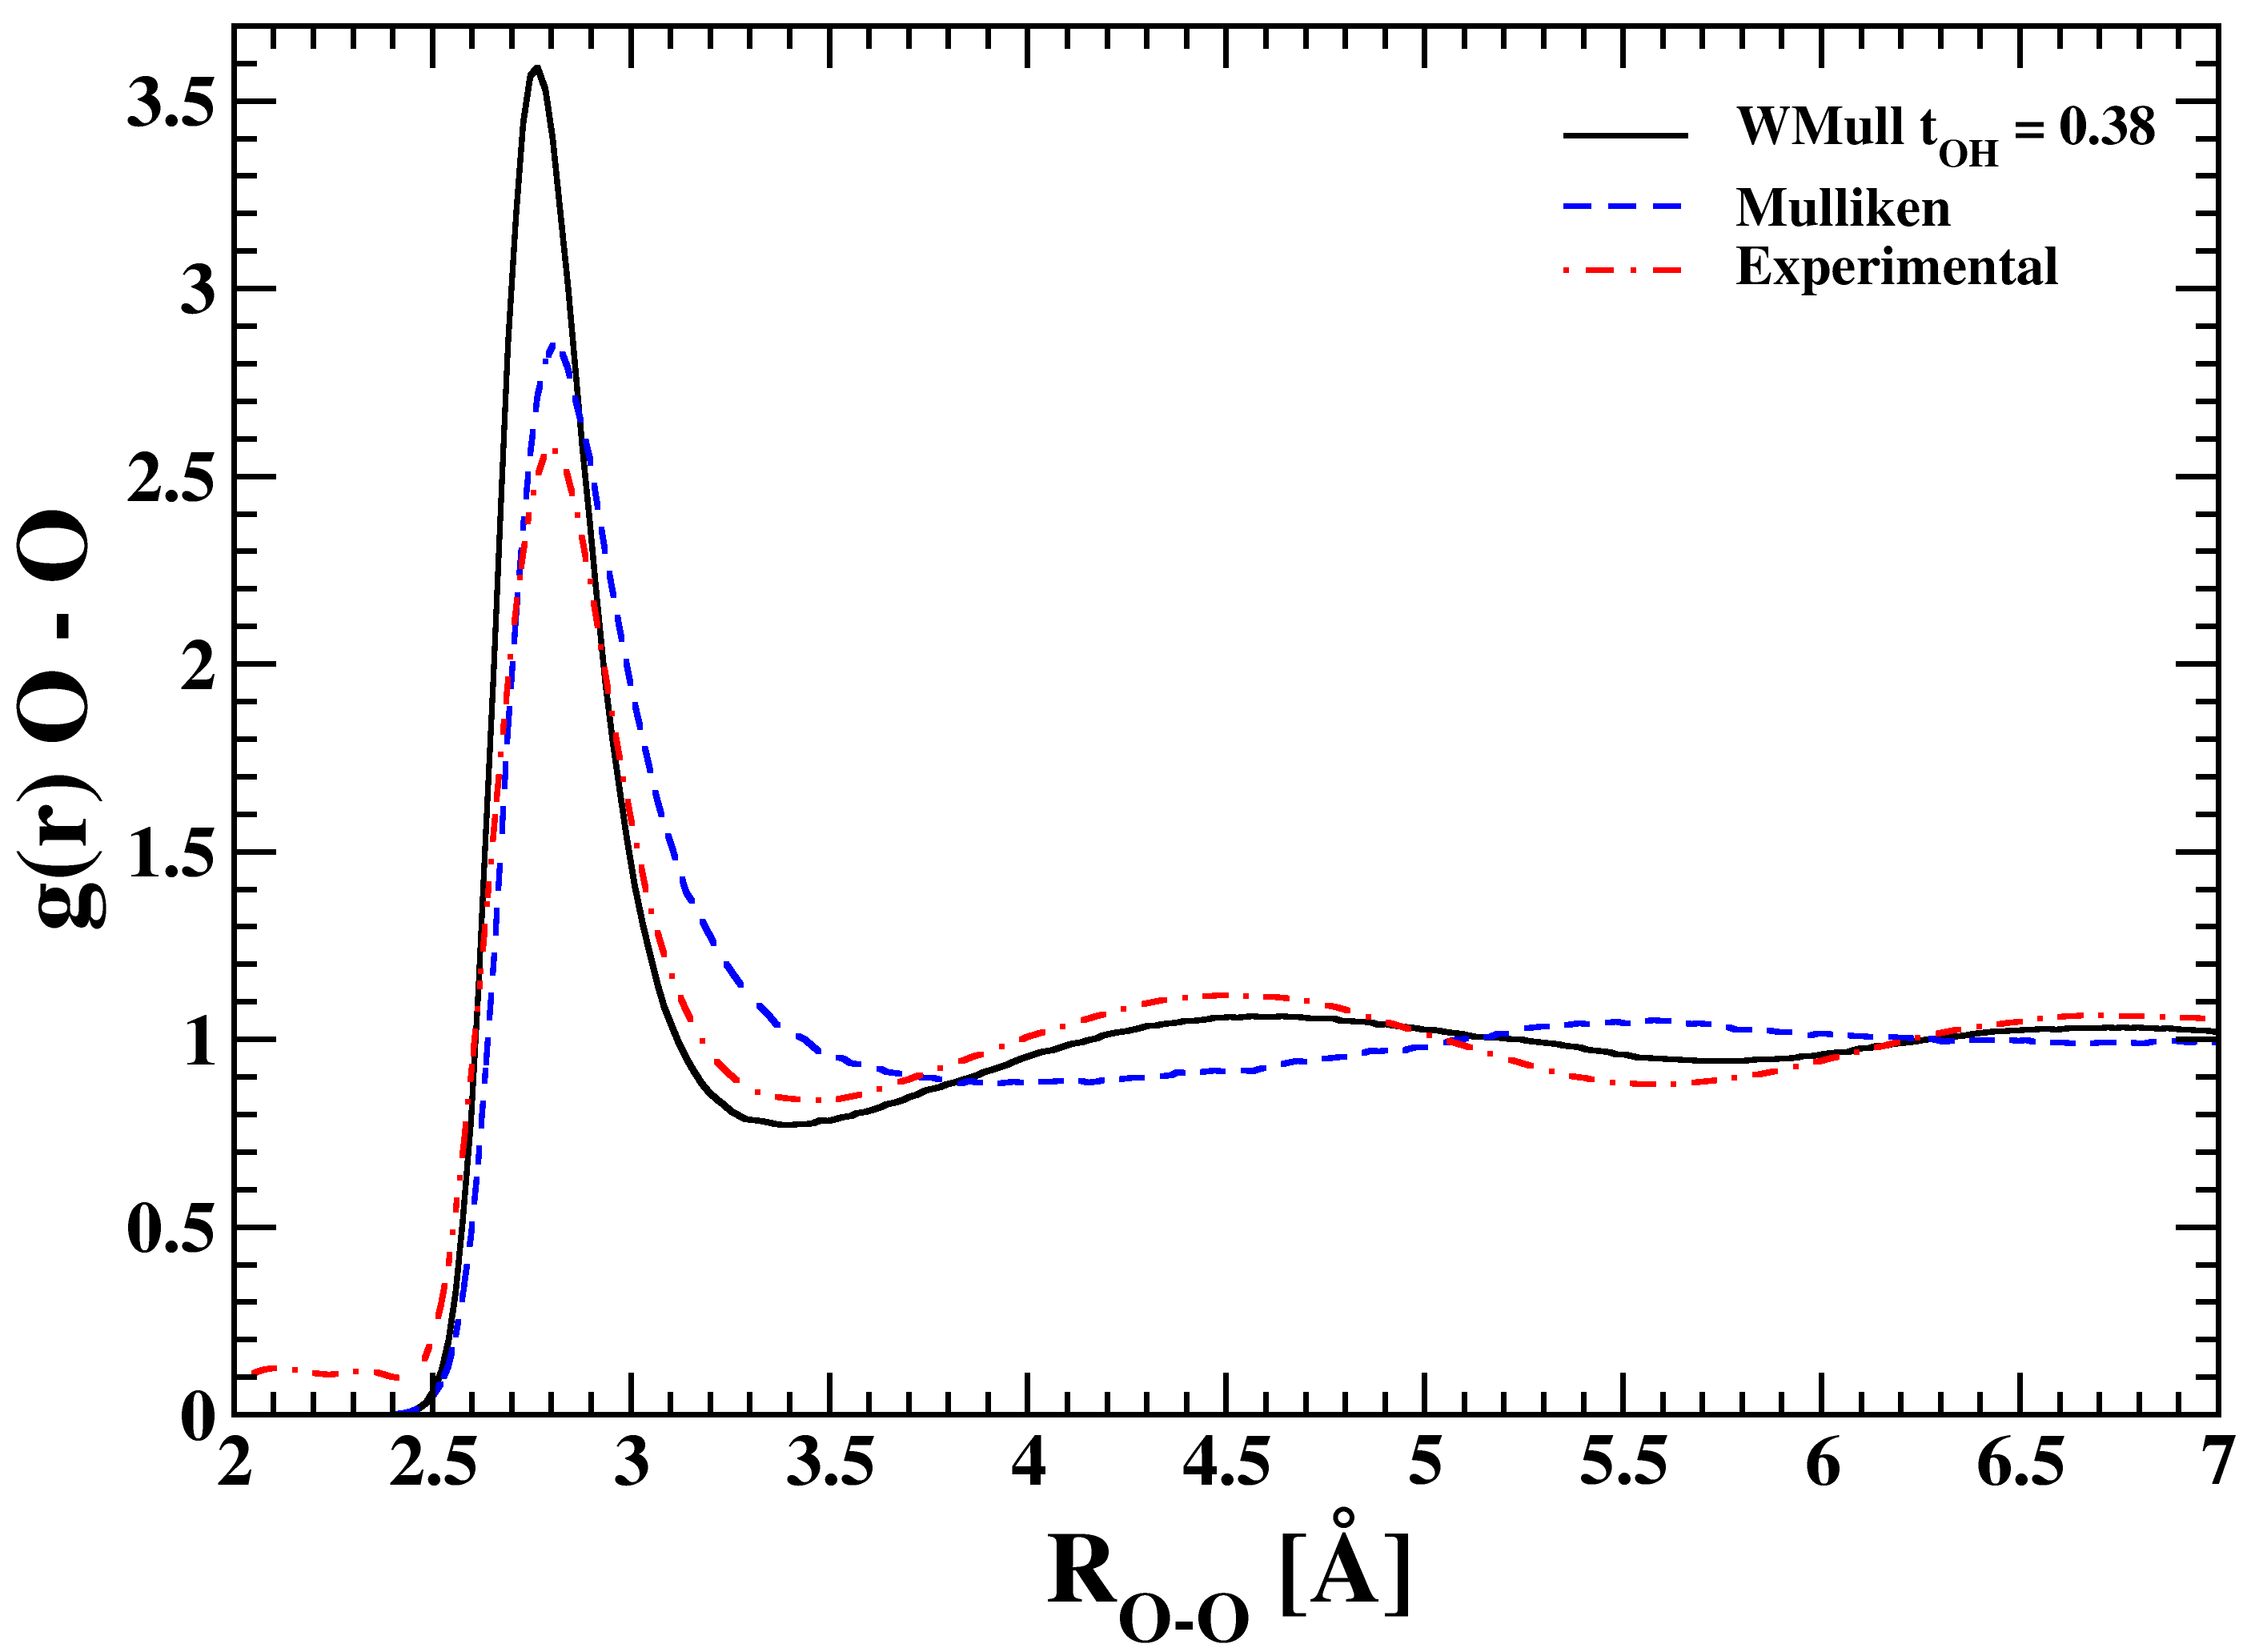
\includegraphics[width=9cm]{liquid_water.png}
\end{center}
\caption{Comparison between the oxygen-oxygen pair radial distribution functions obtained at 300~K for two classical
simulations using the original Mulliken charges and the WMull charges with t$_{OH}$ = 0.39. The experimental 
oxygen-oxygen $g(r)$ obtained by Skinner \textit{et al.} is provided for comparison \cite{Skinner2013}.}
\label{liquidwater}
\end{figure}

\section{Conclusions and perspectives}

In this review, we have presented applications of the SCC-DFTB approach to water clusters, going from fundamental studies (heat capacities,  proton transfer) to applications of paramount importance such as: (i) atmospherical chemistry, in which water clusters constitute a cage where nucleation and particle growth take place, or (ii) astrochemistry, where water ice is expected to act as a catalytic support for a rich heterogeneous (photo) chemistry occurring at the surface of grains in dense media.  In these contexts, theoretical and experimental studies were often achieved in synergy in order to tackle complex issues.

To improve accuracy with respect to experimental measurements or reference theoretical data, the SCC-DFTB calculations we have discussed
 benefited from improvements in the definition of  atomic charges by going beyond the original Mulliken formulation. Once properly defined,
 advantages of the SCC-DFTB approach are manifold: (i) its low computational cost  allows to conduct extensive molecular dynamics simulations in order to explore complex potential energy surfaces or to obtain spectral and thermodynamical properties ; (ii)  its ability to take explicitly into account  the electronic structure allows to study systems in different charge states ; (iii) its transferability enables to investigate a large variety of systems of different chemical nature. This latter point is of paramount importance as the delicate point of this approach is indeed to insure a proper description of  series of systems
 of interest using a unique parametrization of the SCC-DFTB potential. Given the flexibility of the SCC-DFTB parametrization, this is often a much
 easier task than within force field description.

In near future, further applications of the SCC-DFTB approach to water clusters would necessitate
the development and validation of new SCC-DFTB parameters to simulate more complex
systems such as (H$_{2}$SO$_{4}$)$_{n}$(NH$_{3}$)$_{m}$(H$_{2}$O)$_{l}$ clusters which are of
paramount importance in atmospherical processes. This will help in performing simulations closer
to nucleation and condensation conditions found in the  atmosphere and would help in understanding
the formation of aerosols.
Another future application of SCC-DFTB is the description of asphaltene molecules and clusters in a
solvant such as toluene at the interface with liquid water. Understanding the aggregation properties 
of aphaltene molecules at this interface is of paramount importance for oil industry as asphaltenes
are regarded as the most enigmatic component in petroleum. This is due to  their negative influence on
stabilizing the water-in-crude oil emulsion that has deleterious consequences such as plugging
reservoir pores and pipes during oil transportation \cite{asphaltene2015}. These problems are well known to be
closely related to their self-aggregation properties and in recent years, remarkable efforts have been devoted
to study the aggregation of asphaltenes at the water/oil interface. The transferability of the SCC-DFTB
potential will thus allow to study the influence of the nature of the asphaltene (size, presence of aliphatic side chains 
and heteroatoms such as nitrogen or sulfur) and of some other parameters such as solvent nature on 
stabilising asphaltene molecules or clusters at the solvent/water interface. Thermodynamic data
characterizing those systems, for instance desorption free energies, could be obtained using for
instance the umbrella sampling technique. Of course, methodological developments improving
computational efficiency would be useful to achieve such simulations. For instance, algorithms based
on sparse matrix algebra could improve the overall scaling of SCC-DFTB \cite{Scemama2014}.

More chemical reactivity studies should also be considered and  take advantage of biased MD
techniques such as metadynamics \cite{Laio2002,Iannuzzi2003,Laio2005}. This approach has recently
been used in conjunction with SCC-DFTB to study the isomerisation process of the methylenepyrene
cation, a PAH of astrophysical interest \cite{meta_isom}, and of alanine dipeptide in gas and liquid phases
\cite{Cuny2017c}. Finally, following the methodology used to model the reaction of H and CO in section~\ref{reactivity},
more elaborated out-of-equilibrium studies should be considered to understand reactivity in the ISM
and to model particle growth mechanisms in the atmosphere. Such studies would be possible due to
the combination of accuracy and computational efficiency provided by the SCC-DFTB approach which
should still make important contributions to  the understanding of the physical chemistry within water clusters.


\section*{Acknowledgement(s)}

We acknowledge the computing mesocenter CALMIP "Unit\'e Mixte de Service du CNRS" (UMS CNRS 3667)  in Toulouse for generous allocation of computer resources (p0059, p1320 and p17002). 

%\section*{Disclosure statement}

%An unnumbered section, e.g.\ \verb"\section*{Disclosure statement}", may be used to declare any potential conflict of interest and included \emph{in the non-%anonymous version} before any Notes or References, after any Acknowledgements and before any Funding information.

\section*{Funding}

This work has been funded by the Agence Nationale de la Recherche (ANR) project "PARCS'' ANR-13-BS08-0005 "PARCS (Polycyclic Aromatic Hydrocarbons Reactivity in Cryogenic Solids)", with support from the French research network EMIE (Edifices Mol\'{e}culaires Isol\'{e}s et Environn\'{e}s, GDR 3533 of CNRS). It has also been partially
supported through the NEXT grant No. ANR-10-LABX-0037 in the framework of the "Programme des Investissements d'Avenir". 


%\section*{Notes on contributor(s)}

%An unnumbered section, e.g.\ \verb"\section*{Notes on contributors}", may be included \emph{in the non-anonymous version} if required. A photograph may be added if requested.


%\section*{Nomenclature/Notation}

%An unnumbered section, e.g.\ \verb"\section*{Nomenclature}" (or \verb"\section*{Notation}"), may be included if required, before any Notes or References.

%\section*{Notes}

%An unnumbered `Notes' section may be included before the References (if using the \verb"endnotes" package, use the command \verb"\theendnotes" where the notes are to appear, instead of creating a \verb"\section*").

%\begin{verbatim}
\bibliographystyle{tfnlm}
\bibliography{biblio_water}
%\end{verbatim}

\end{document}
